As indicated in Figure~\ref{fig:sigRegionBG}, different Standard Model processes contribute to the event sample in the signal region. To distinguish a potential signal from these backgrounds, a precise estimation of the background contributions is mandatory. While the simulation of these processes and the response of the CMS detector gives a good description of the data for the majority of the phase space, a large number of uncertainty sources are introduced in the modelling of the physical process and the detector. Therefore a higher precision can be achieved by deriving the background estimates directly from the recorded data. The background processes are categorized as either being flavour-symmetric or as containing the production of a Z boson. A dedicated method is applied for each of the two categories. The different background processes are:

\section{Flavour-symmetric backgrounds}
Processes that are symmetric in the production of same-flavour and opposite-flavour lepton pairs allow for the estimation of their contribution to the SF event sample from the OF one. The most dominant of these processes is the dileptonic decay of top-pair production, where the leptons are produced uncorrelatedly in the decay of the W bosons. Other examples are the decays of two $\tau$ leptons, which are in turn produced in the decay of a Z boson or the dileptonic decay of W pairs. Another contribution to this class of backgrounds are misidentified leptons, as will be demonstrated later. 

No significant deviation from flavour-symmetry has been observed in the decays of the W boson, with a measured ratio of the branching fractions into $e+\nu$ and $\mu + \nu$ of $1.007\pm0.021$. In the decays of the $\tau$ lepton the different masses of electron and muon have a noticeable effect, resulting in a slightly favoured decay into electrons. Here the ratio of branching fractions is $1.0241\pm0.0032$~\cite{PDG}. As backgrounds with $\tau$ leptons are a sub-dominant contribution to the the flavour-symmetric backgrounds, these can be considered to be fully flavour-symmetric on particle level. However, distortions of the flavour-symmetry are introduced by the different efficiencies for triggering, reconstructing, and identifying electrons and muons in CMS. The background estimation from OF events therefore has to include a correction for this deviation, which is applied as a multiplicative factor:
\begin{equation}
N_{SF}^{pred} = \Rsfof \cdot N_{OF}.
\end{equation}
Two independent methods are utilized to measure \Rsfof on data. In the first approach is is directly measured as the ratio of SF to OF events in the control region for flavour-symmetric backgrounds. The second approach studies the lepton efficiencies and derives \Rsfof factorized into the effects of trigger efficiencies and reconstruction and identification efficiencies.  

\subsection{Direct measurement of \Rsfof}
The ratio of SF to OF events as a function of \mll in simulation is shown in Figure~\ref{fig:controlRatioMC}, separately for the central and forward lepton selection. The ratio is close to one, independent of \mll, allowing for the same value of \Rsfof to be applied over the full mass range. In data however there are contributions from non-flavour-symmetric processes containing Z bosons at the Z peak. Therefore the on-Z mass bin is excluded from the calculation and only events in the mass regions $\unit{20}{\giga\electronvolt}< \mll < \unit{70}{\giga\electronvolt}$ and $\mll > \unit{120}{\giga\electronvolt}$ are considered.   	
\begin{figure}
\begin{center}
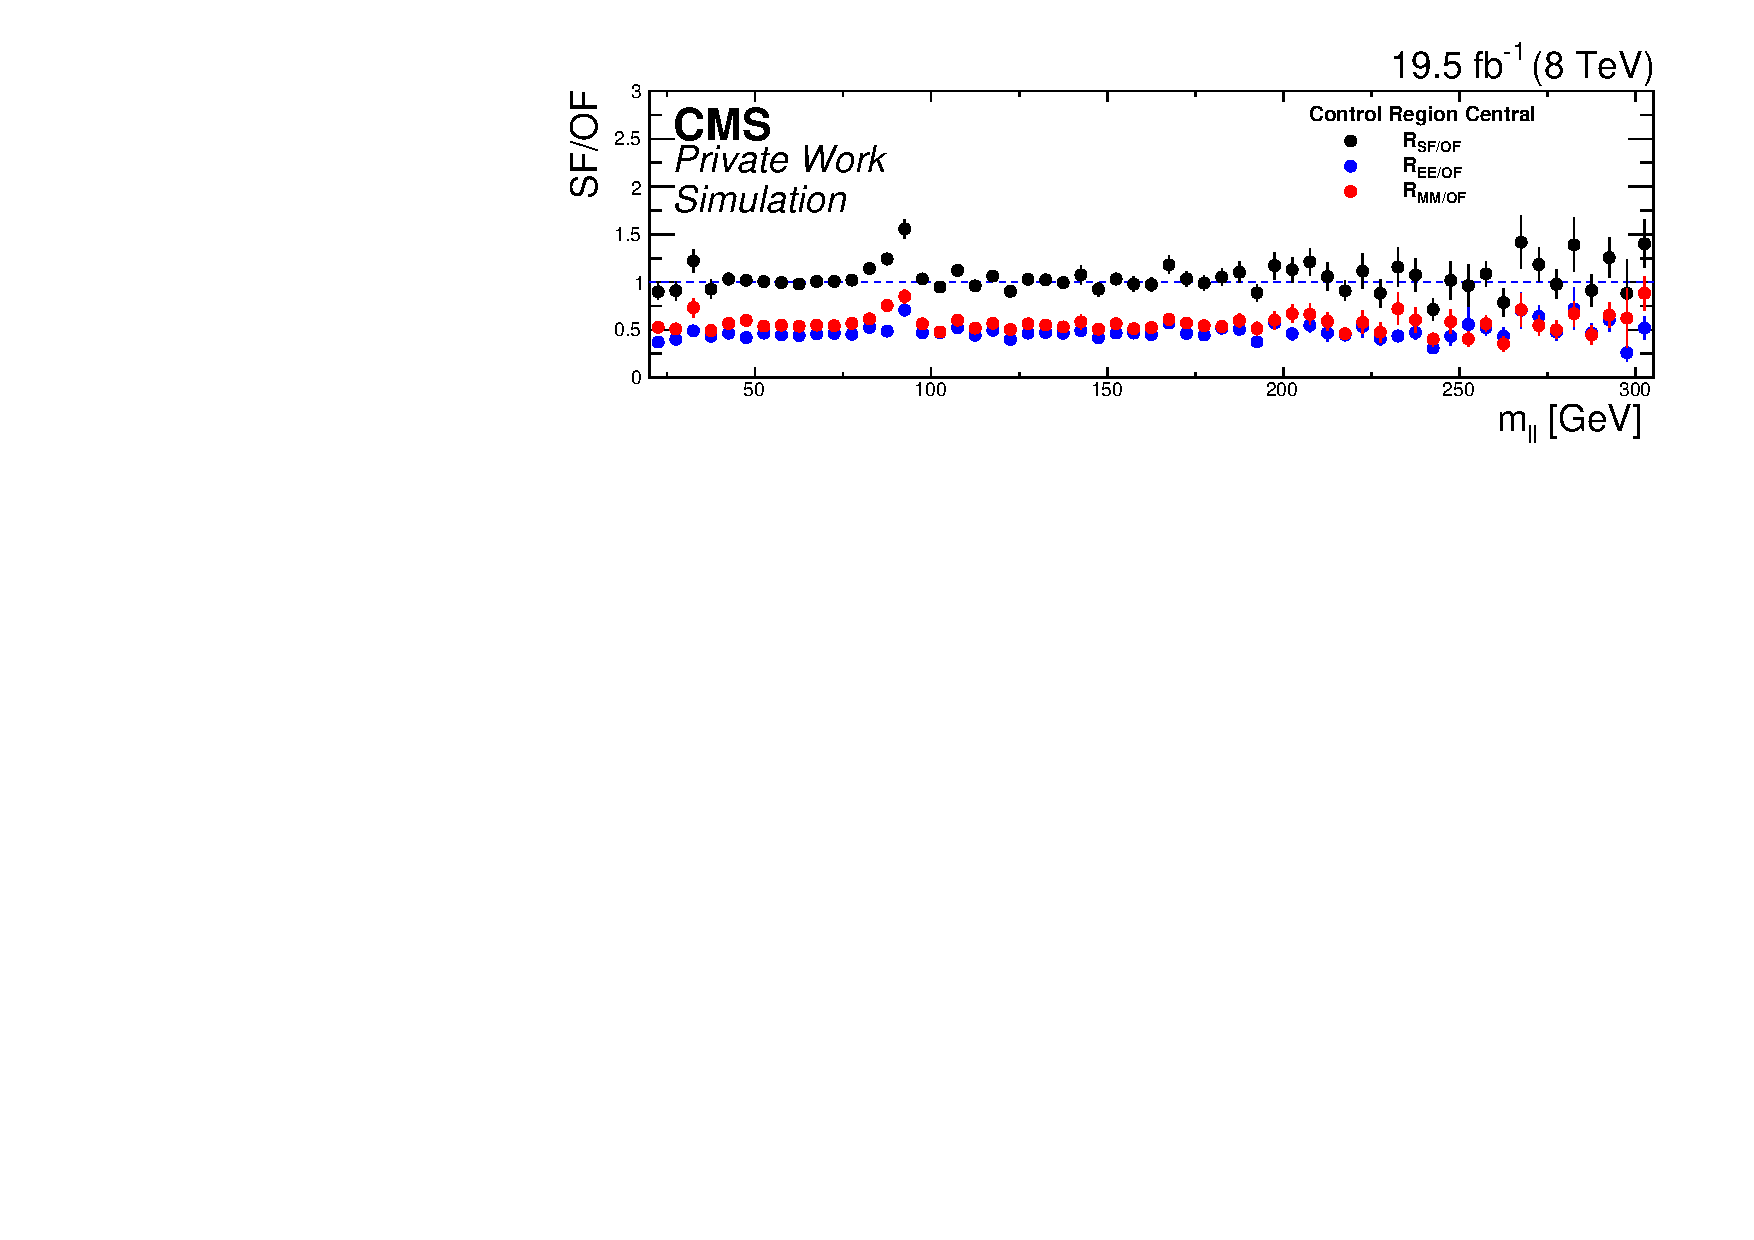
\includegraphics[scale=0.35]{plots/BG/control/rSFOF_ControlCentral_Full2012_Mll_None_MC.pdf}\\
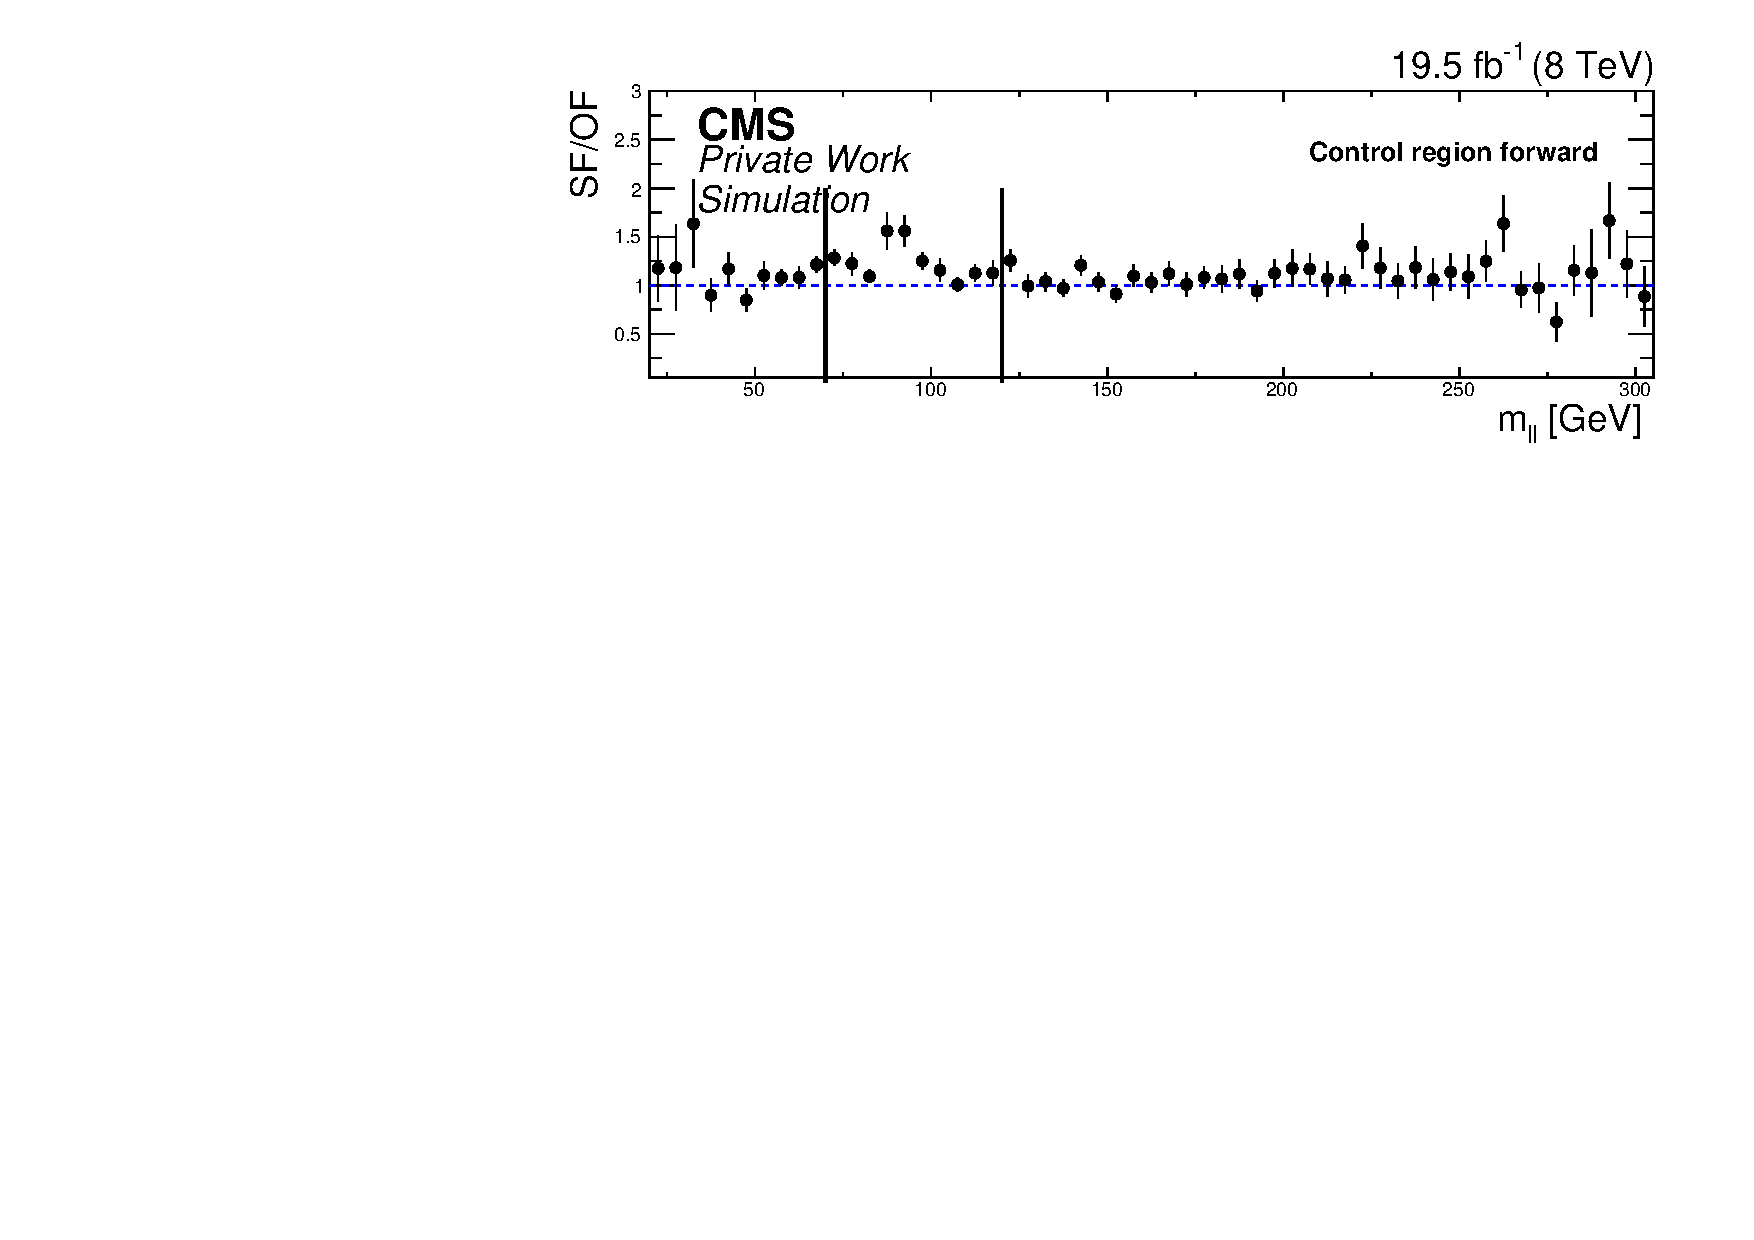
\includegraphics[scale=0.35]{plots/BG/control/rSFOF_ControlForward_Full2012_Mll_None_MC.pdf}
\caption{Ratio of SF to OF events as a function of \mll in the $t\bar{t}$ control region for the dileptonic $t\bar{t}$ sample. Shown are the results for the central (top) and forward (bottom) lepton selection.}
\label{fig:controlRatioMC}
\end{center}
\end{figure}
The observed ratio on data as a functions of \mll is shown in Figure~\ref{fig:controlRatio}. No dependence on \mll is observed.
\begin{figure}
\begin{center}
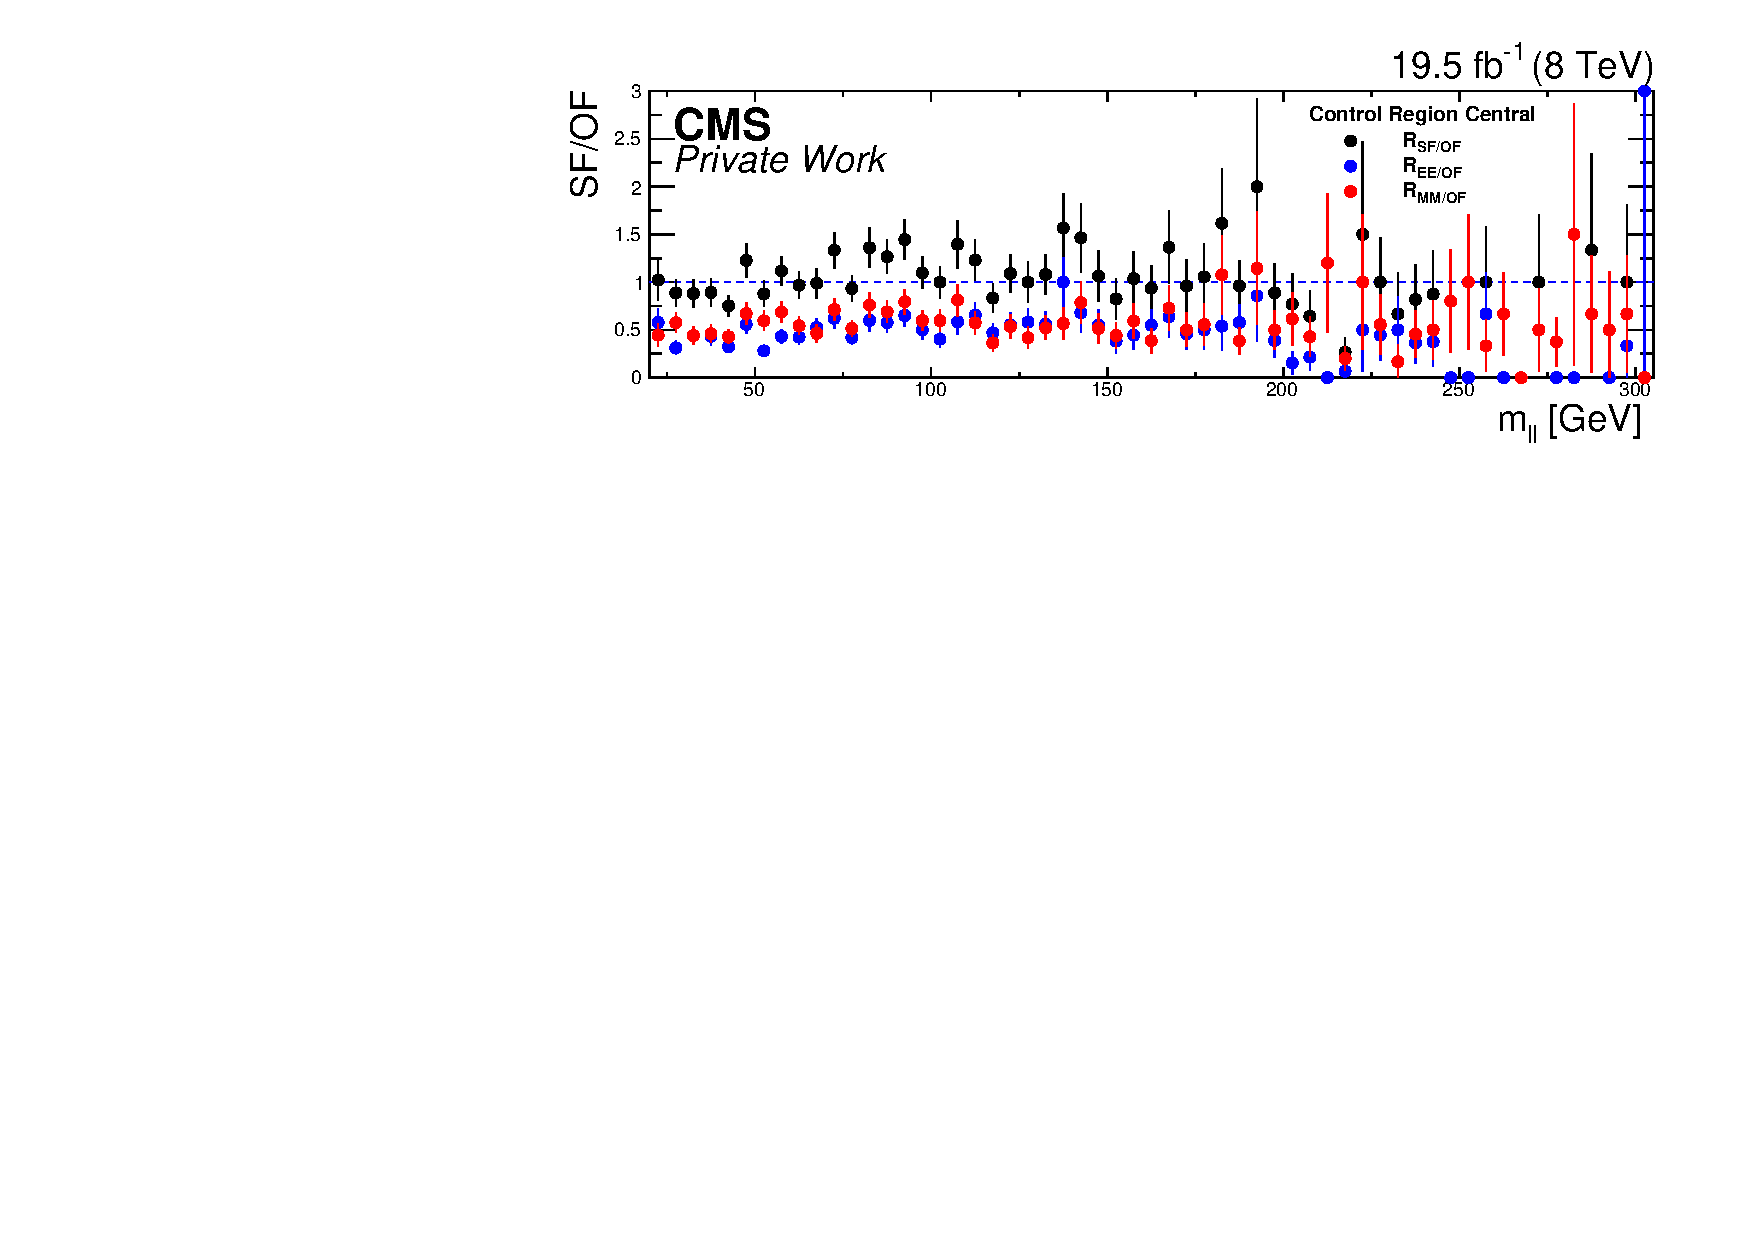
\includegraphics[scale=0.35]{plots/BG/control/rSFOF_ControlCentral_Full2012_Mll_None.pdf}\\
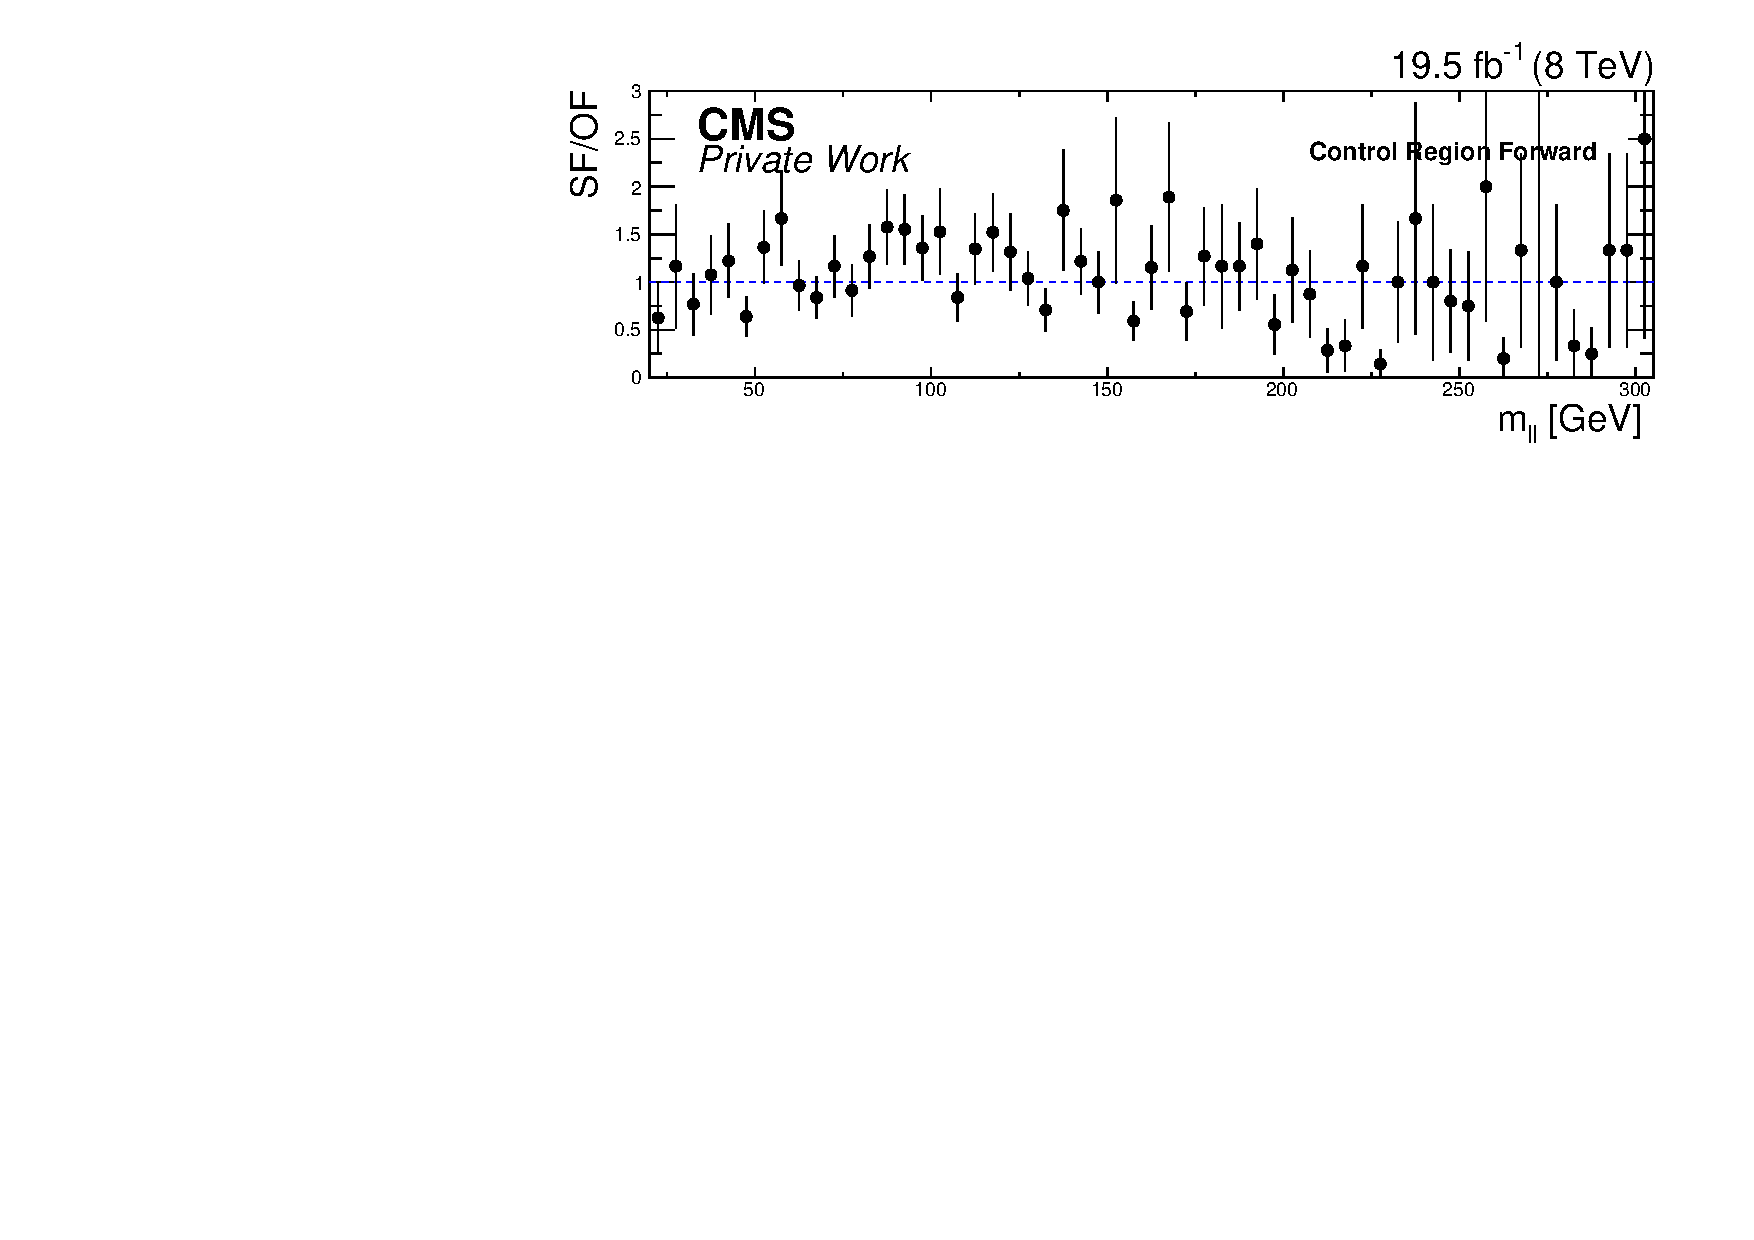
\includegraphics[scale=0.35]{plots/BG/control/rSFOF_ControlForward_Full2012_Mll_None.pdf}
\caption{Ratio of SF to OF events as a function of \mll in the $t\bar{t}$ control region on data. Shown are the results for the central (top) and forward (bottom) lepton selection.}
\label{fig:controlRatio}
\end{center}
\end{figure}
The numerical results are summarized in Table~\ref{tab:rsofControl}


\begin{table}[hbtp]
 \renewcommand{\arraystretch}{1.3}
 \setlength{\belowcaptionskip}{6pt}
 \centering
 \caption{Observed event yields in the control region and the resulting values of \Rsfof, \Reeof, and \Rmmof. The results are shown separately for the central and forward lepton selection and the same quantities derived on simulation are shown for comparison. For the simulation, the ratio between the values of \Rsfof, \Reeof, and \Rmmof measured in the signal and control region is shown.}
  \label{tab:rSFOF}
\begin{tabular}{l|c|c|c|c}
\multicolumn{5}{c}{Control region}\\ \hline     
 & $N_{SF}$ & $N_{OF}$ & $ \Rsfof \pm \sigma_{stat}$ & signal/control region $\pm \sigma_{stat}$  \\    
\hline
&  \multicolumn{4}{c}{Central} \\
\hline
 Data & 1458 & 1448 & 1.007$\pm$0.037 & -- \\
 MC & 1484.2 & 1436.1 & 1.034$\pm$0.015 & 1.016$\pm$0.020\\
 
 
    \hline 
& \multicolumn{4}{c}{Forward} \\
\hline
 Data & 545 & 537 & 1.015$\pm$0.062 & -- \\
 MC & 565.1 & 517.5 & 1.092$\pm$0.026 & 0.997$\pm$0.034\\

\hline\hline
 & $N_{ee}$ & $N_{OF}$ & $ \Reeof \pm \sigma_{stat}$ & signal/control region $\pm \sigma_{stat}$  \\    
\hline
&  \multicolumn{4}{c}{Central} \\
\hline
 Data & 663 & 1448 & 0.458$\pm$0.021 & -- \\
 MC & 670.0 & 1436.1 & 0.467$\pm$0.008 & 1.017$\pm$0.025\\
 
 
    \hline 
& \multicolumn{4}{c}{Forward} \\
\hline
 Data & 239 & 537 & 0.445$\pm$0.035 & -- \\
 MC & 237.9 & 517.5 & 0.460$\pm$0.014 & 1.023$\pm$0.043\\

\hline\hline
 & $N_{\mu\mu}$ & $N_{OF}$ & $ \Rmmof \pm \sigma_{stat}$ & signal/control region $\pm \sigma_{stat}$  \\    
\hline
& \multicolumn{4}{c}{Central} \\
\hline
 Data & 795 & 1448 & 0.549$\pm$0.024 & -- \\
 MC & 814.2 & 1436.1 & 0.567$\pm$0.010 & 1.015$\pm$0.025\\
 
 
    \hline 
 & \multicolumn{4}{c}{Forward} \\
\hline
 Data & 306 & 537 & 0.570$\pm$0.041 & -- \\
 MC & 327.3 & 517.5 & 0.632$\pm$0.018 & 0.978$\pm$0.039\\

  
\end{tabular}  
\end{table}


\subsection{Determination of \Rsfof with the factorization method}
\label{sec:rmue}
Asymmetries between the lepton flavours introduced by differing reconstruction and selection efficiencies can be corrected for if the ratio of efficiencies for muons and electrons $\rmue = \frac{\epsilon_{\mu}}{\epsilon_{e}}$ is known. Under the assumption that the efficiencies for the two leptons in the event factorize, i.e. $\epsilon_{ll} = \epsilon_{l}\cdot\epsilon_{l}$, the number of dielectron and dimuon events can be estimated from the opposite-flavour events using the relations
\begin{equation}
n_{ee}^{*} = \frac{1}{2}\cdot \frac{n_{OF}^{*}}{\rmuestar}
\end{equation}
and 
\begin{equation}
n_{\mu\mu}^{*} = \frac{1}{2} \cdot \rmuestar \cdot n_{OF}^{*},
\end{equation}
the $^{*}$ indicating that these are the values unaffected by trigger efficiencies.
The prediction of the combined same-flavour yield is therefore given by
\begin{equation}
n_{SF}^{*} = \frac{1}{2}\cdot \left( \rmuestar + \frac{1}{\rmuestar} \right) n_{OF}^{*}.
\end{equation}
In practice, all measured quantities are affected by the efficiencies of the different dilepton triggers. The measured number of SF events will therefore be
\begin{equation}
n_{SF} = \effeet \cdot n_{ee}^{*} + \effmmt \cdot n_{\mu\mu}^{*},
\end{equation}
where $\epsilon_{ll}^T$ denotes the trigger efficiency for the given dilepton combination.\\
Also the predictions for $n_{ee}^{*}$ and $n_{\mu\mu}^{*}$ have to include the trigger efficiencies. Here \rmuestar is expressed in terms of the measured value \rmue, which is derived from the \EE and \MM event yields in the Drell-Yan control region (see Section~\ref{sec:rmue}) as 
\begin{equation}
\rmue  = \sqrt{\frac{N_{\mu\mu}}{N_{ee}}} \approx \sqrt{\frac{\epsilon_{\mu}^2 \effmmt}{\epsilon_{e}^2 \effeet}} = \rmuestar \cdot \sqrt{\frac{\effmmt}{\effeet}}.
\end{equation}
Taking into account also that the measured event yield in the OF channel is $n_{OF} = \effemt \cdot n_{OF}^{*}$, the estimate for the yields in the same-flavour channel becomes
\begin{equation}
n_{ee} = \frac{1}{2\rmue} \cdot \frac{\sqrt{\effeet \effmmt}}{\effemt} n_{OF} = \Reeof n_{OF}
\label{eq:nee}
\end{equation} 
and
\begin{equation}
n_{\mu\mu} = \frac{1}{2}\rmue  \cdot \frac{\sqrt{\effeet \effmmt}}{\effemt} n_{OF} = \Rmmof n_{OF}.
\label{eq:nmm}
\end{equation} 
Finally, the combined prediction of the SF yield is
\begin{equation}
n_{SF} = \frac{1}{2}\left(\rmue + \frac{1}{\rmue}\right) \cdot \frac{\sqrt{\effeet \effmmt}}{\effemt}  n_{OF} = \Rsfof n_{OF}.
\label{eq:nsf}
\end{equation}
\subsubsection{Measurement of \rmue}
The measurement of \rmue is performed in the Drell-Yan control region as the ratio of \MM to \EE events on the Z peak, requiring $\unit{60}{\giga\electronvolt} < \mll < \unit{120}{\giga\electronvolt}$. A comparison of the recorded data to the different contributions  from Standard Model processes, estimated from simulation, is shown in Figure~\ref{fig:rmueMll}. The Drell-Yan process is the dominating source of events in this selection. Good agreement between data and simulation is observed, indicating a good understanding of this kinematic region by CMS.   
\begin{figure}[htbp]
\centering
\begin{minipage}[t]{0.49\textwidth}
  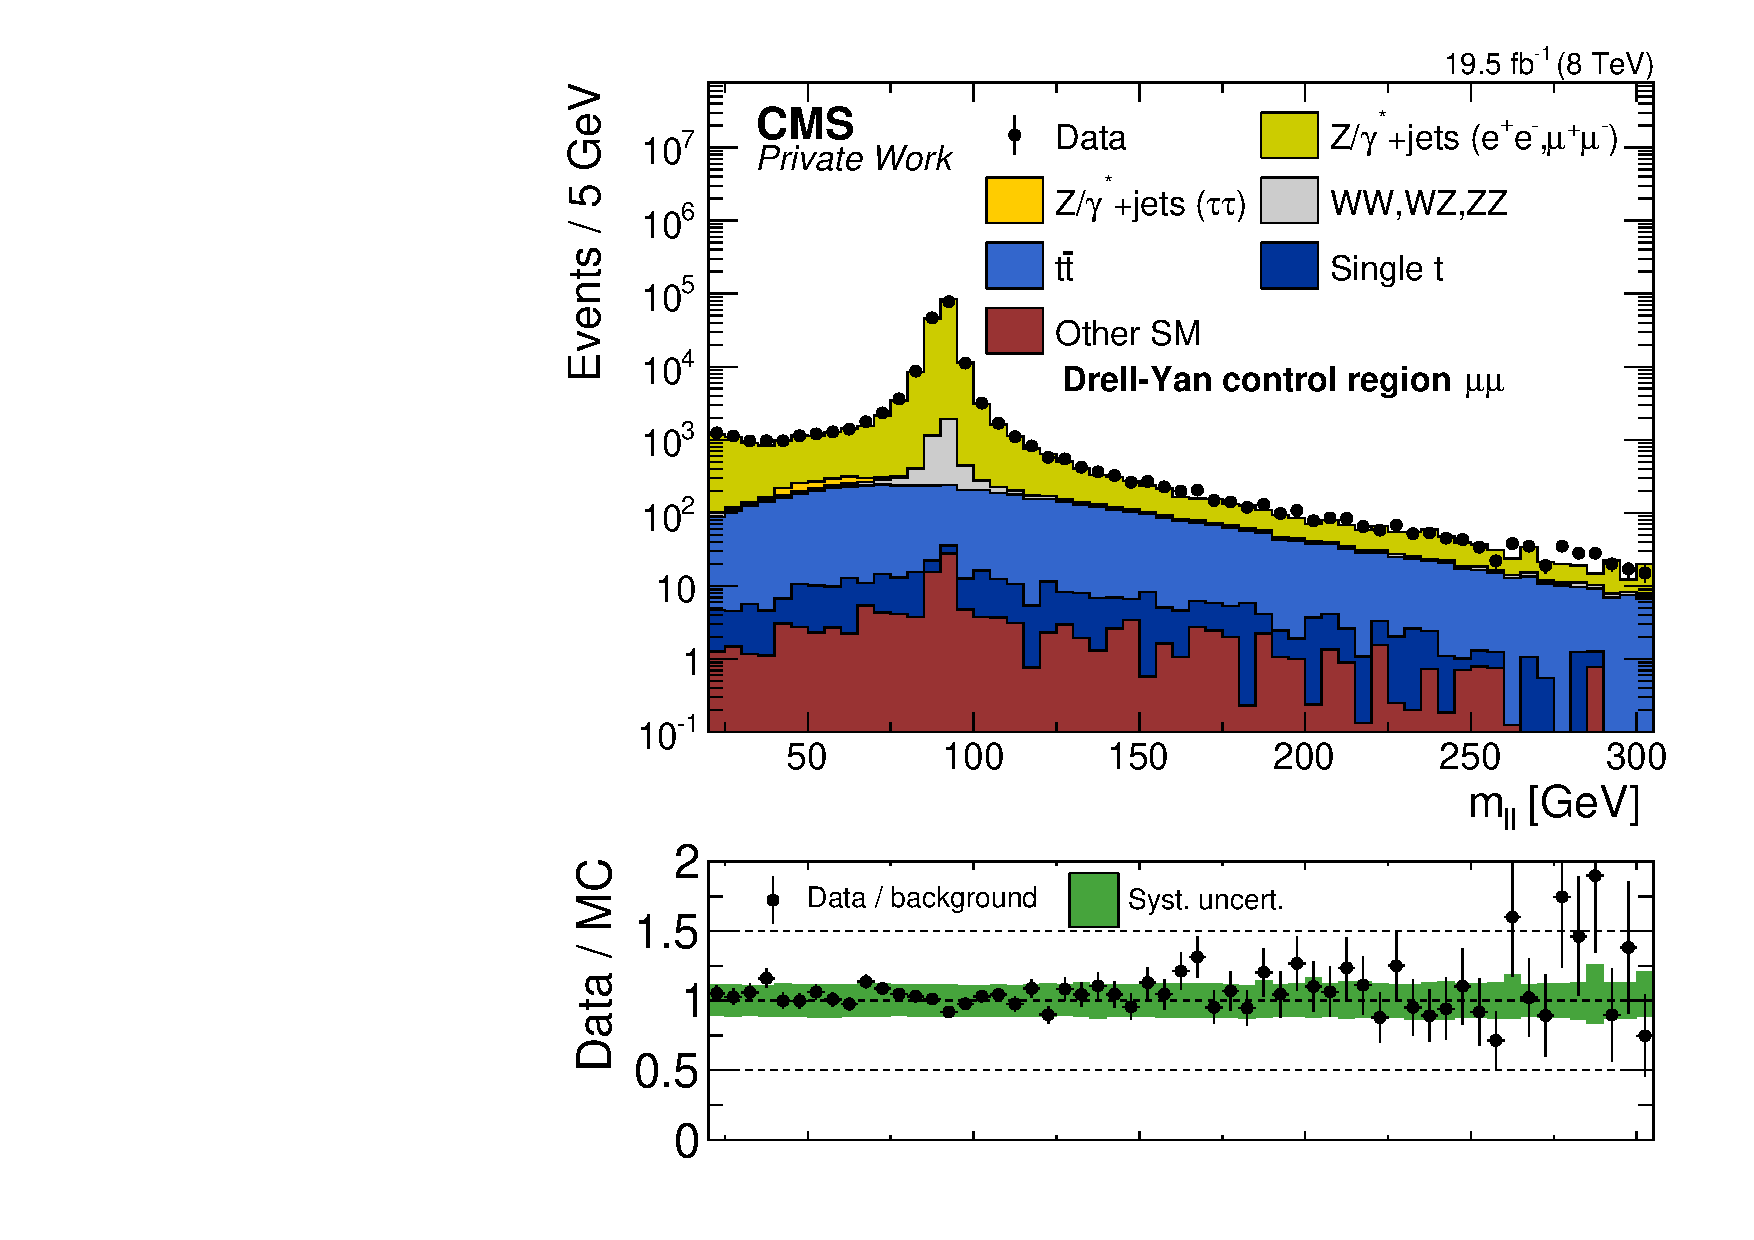
\includegraphics[width=\textwidth]{plots/BG/rmue/DrellYanControl_Mll_Full2012_MuMu_TopReweighted.pdf}
\end{minipage}
\begin{minipage}[t]{0.49\textwidth}
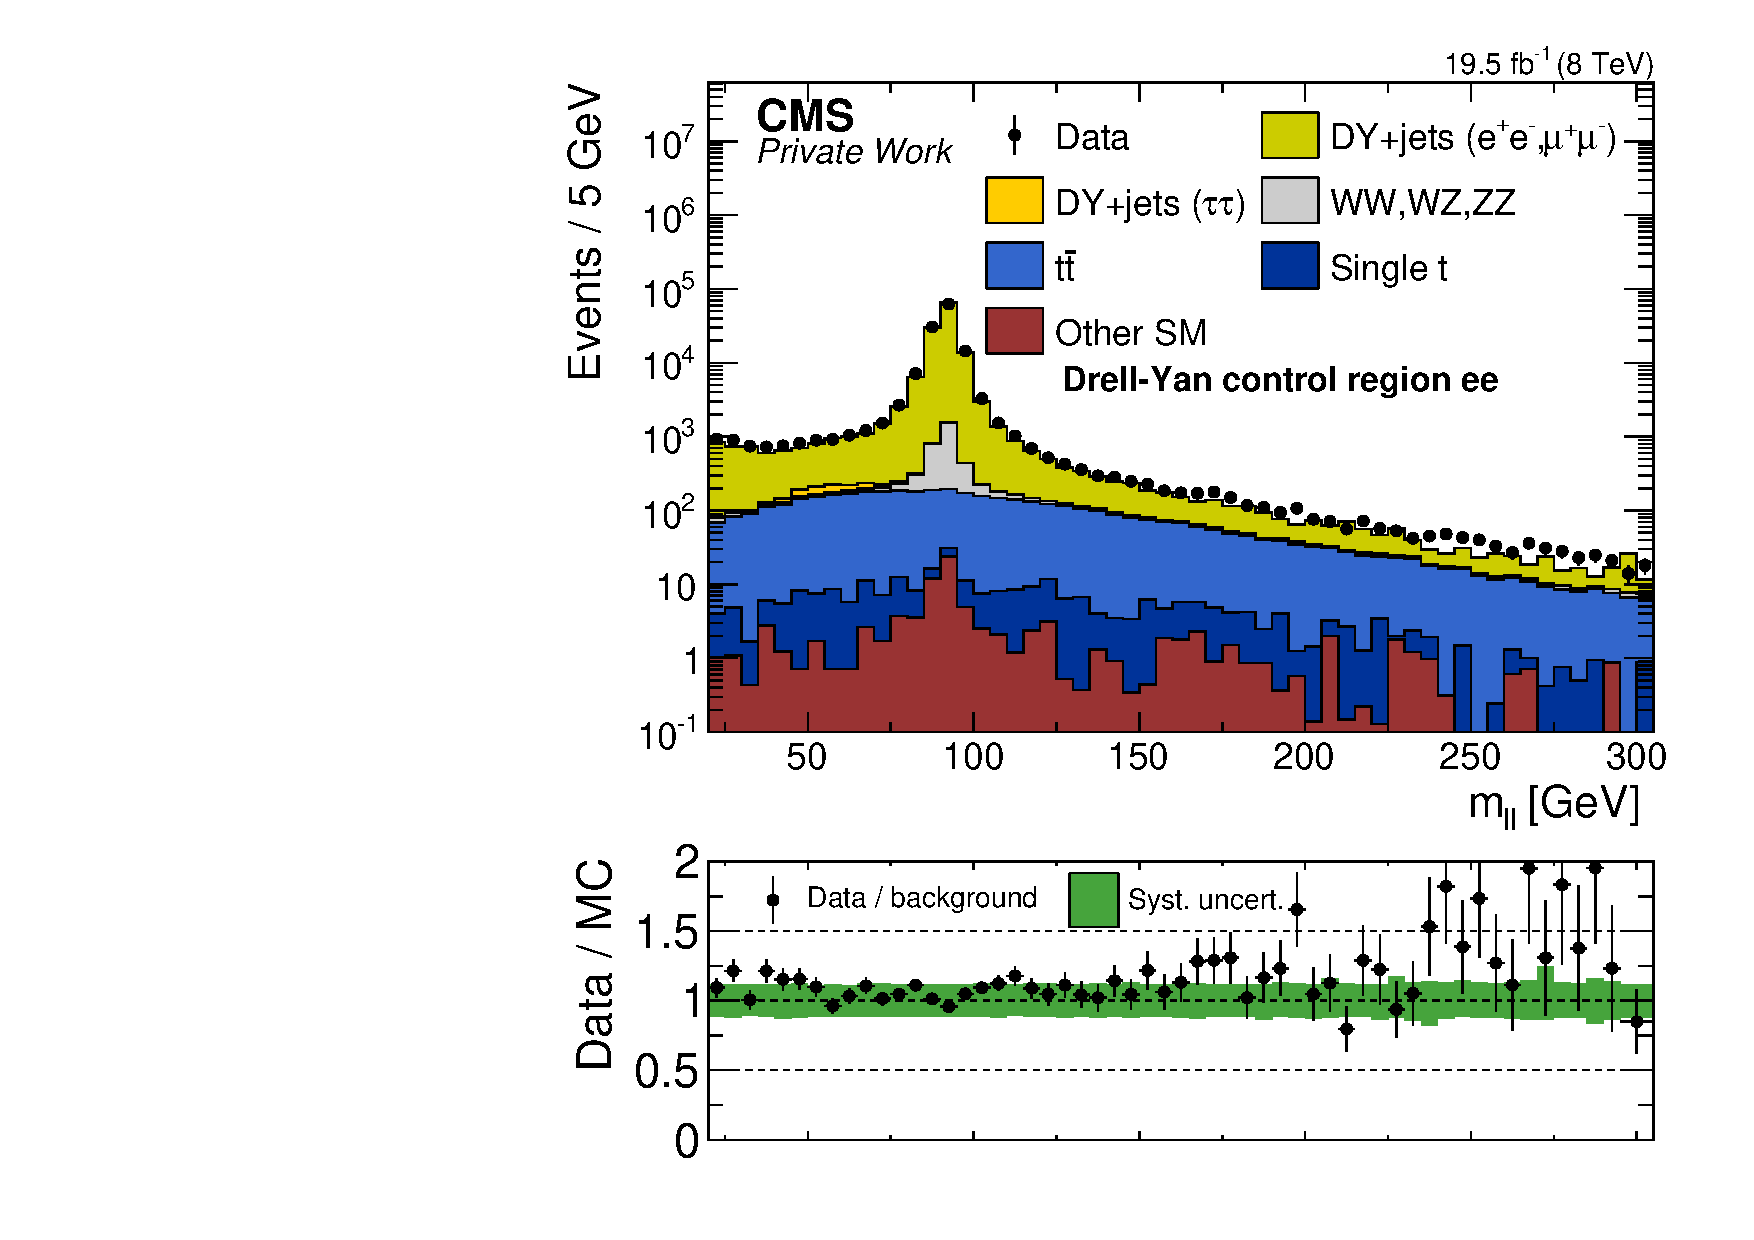
\includegraphics[width=\textwidth]{plots/BG/rmue/DrellYanControl_Mll_Full2012_EE_TopReweighted.pdf}
\end{minipage}
\caption{Distribution of \mll in the Drell-Yan control region for \MM events (left) and \EE events (right). The data is shown as the black dots, while the contributions from Standard Model processes, estimated from simulation, are shown as the stacked histograms.}
\label{fig:rmueMll}
\end{figure} 
The results of the calculation of \rmue are shown in Table~\ref{tab:RValuesControl}. Given are the observed yields for \MM and \EE events and the resulting value of \rmue with statistical and systematic uncertainties. In the central lepton selection, the \MM yield is about 18\% higher than the \EE yield. Similar results are observed on Drell-Yan simulation. For events with leptons in the forward region, a larger asymmetry between muons and electrons is observed, here the \MM yield is about 40\% higher than the \EE yield. 

\begin{table}[hbtp]
 \renewcommand{\arraystretch}{1.3}
 \setlength{\belowcaptionskip}{6pt}
 \centering
 \caption{Result of the calculation of \rmue. Shown are the observed event yields in the Drell--Yan control region for the central and forward lepton selection in the \EE and \MM channels and the resulting values of 
\rmue. The same quantaties derived from simulation are shown for comparison.}
  \label{tab:rMuE}
  \begin{tabular}{l| ccc }

    							& $N_{\mu\mu}$ &  $N_{ee}$ & $\rmue \pm \sigma_{\text{stat.}} \pm \sigma_{\text{syst.}}$ \\ 
    
    \hline
    							& \multicolumn{3}{c}{Central}  \\ 

    \hline
        Data       &  98284                   & 83035              &  1.09$\pm$0.01$\pm$0.11    \\

        MC       &  99719                   & 82035              &  1.10$\pm$0.00$\pm$0.11    \\

\hline
    							& \multicolumn{3}{c}{Forward}  \\ 

    \hline
        Data       &  62212                   & 44437              &  1.18$\pm$0.01$\pm$0.24    \\

        MC       &  66327                   & 45541              &  1.21$\pm$0.00$\pm$0.24    \\

  \end{tabular}
\end{table}



The systematic uncertainties of the measurement 10\% for the central and 20\% for the forward lepton selection. These values are obtained from studies of the dependency of \rmue on relevant observables. These are on the one hand properties of the lepton pairs, while on the other hand the jet multiplicity and \MET are studied to asses potential biases introduced when applying \Rsfof in the signal region. The dependencies of \rmue on \mll, \MET, and $N_{jets}$ are shown in Figure~\ref{fig:rmueDependencies}. Some dependency is observed in the case of \mll, where the values are higher for low \mll below the Z peak. This can be traced back to a dependency on the \pt of the leptons, where the efficiency for muons has a sharper turnon compared to electrons, for example for the dilepton triggers. In data, there is a strong effect visible around the Z peak for forward leptons. This is caused by a systematic shift of the position of the Z peak between electron and muons and is not a general property of \rmue, as is evident from the comparison with $t\bar{t}$ simulation shown in the upper right of Figure~\ref{fig:rmueDependencies}. No strong dependencies can be observed for \MET and $N_{jets}$ within the statistical uncertainties. All observed deviations from the central values are covered by the systematic uncertainties assigned to the measurement. Further information on the dependency studies can be found in Appendix~\ref{app:rmue}
\begin{figure}[htbp]
\centering
\begin{minipage}[t]{0.49\textwidth}
  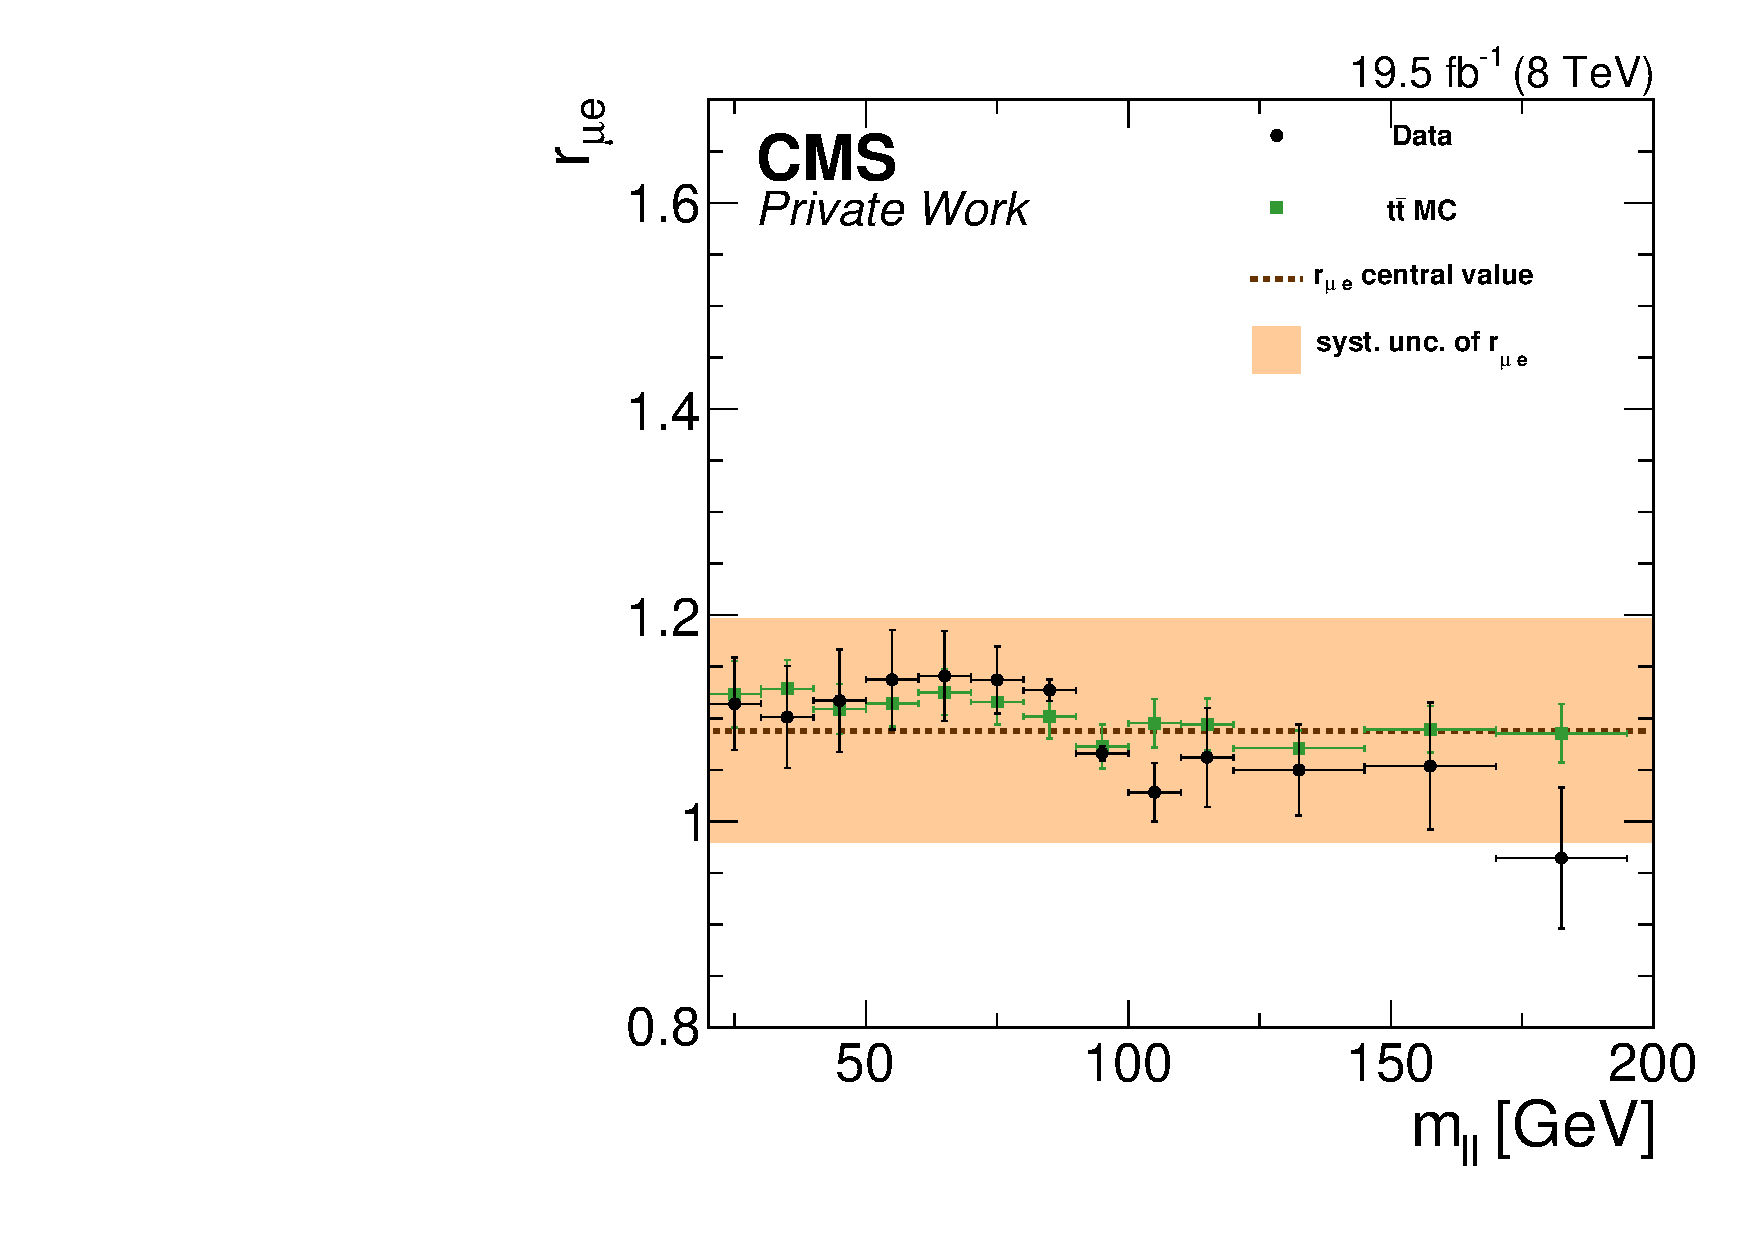
\includegraphics[width=\textwidth]{plots/BG/rmue/rMuE_ZPeakControlCentral_Full2012_Mll_None.pdf}
\end{minipage}
\begin{minipage}[t]{0.49\textwidth}
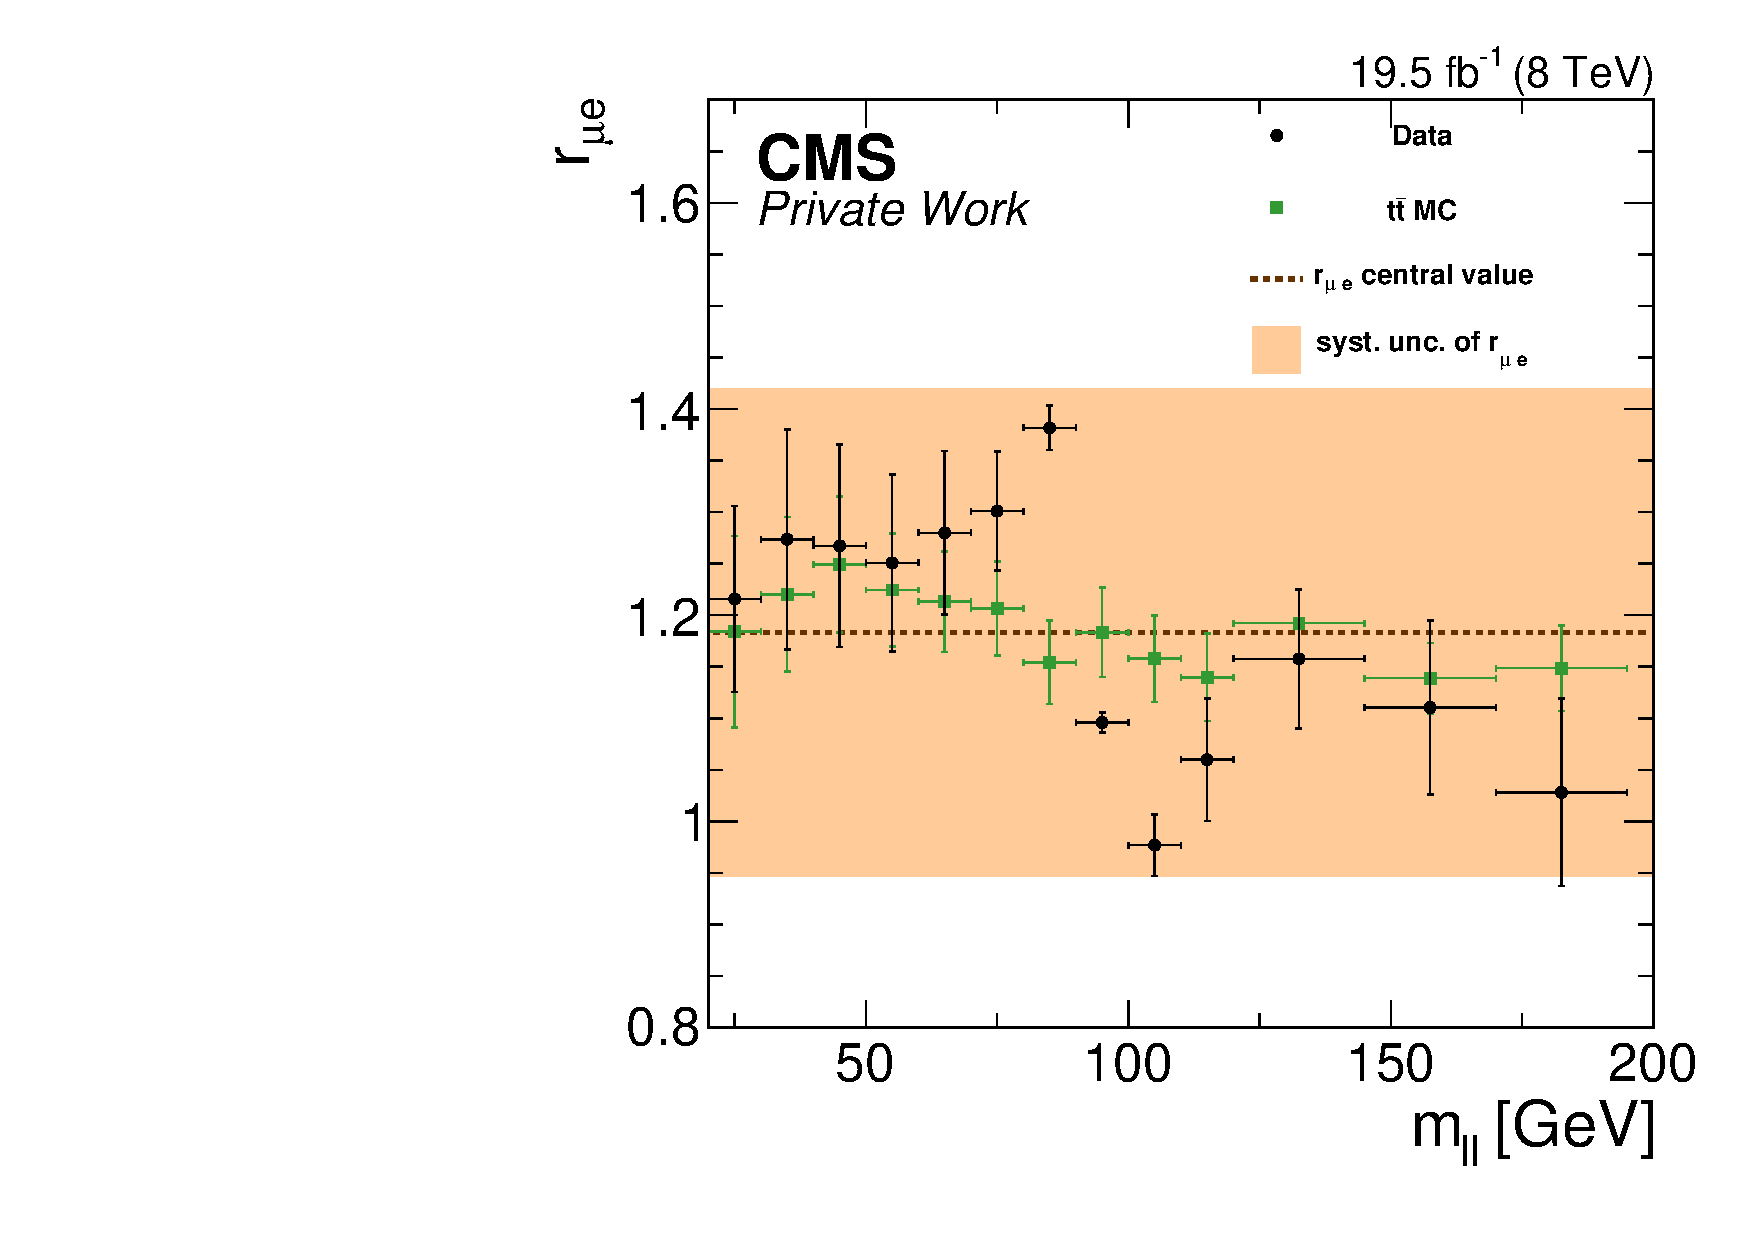
\includegraphics[width=\textwidth]{plots/BG/rmue/rMuE_ZPeakControlForward_Full2012_Mll_None.pdf}
\end{minipage}
\begin{minipage}[t]{0.49\textwidth}
  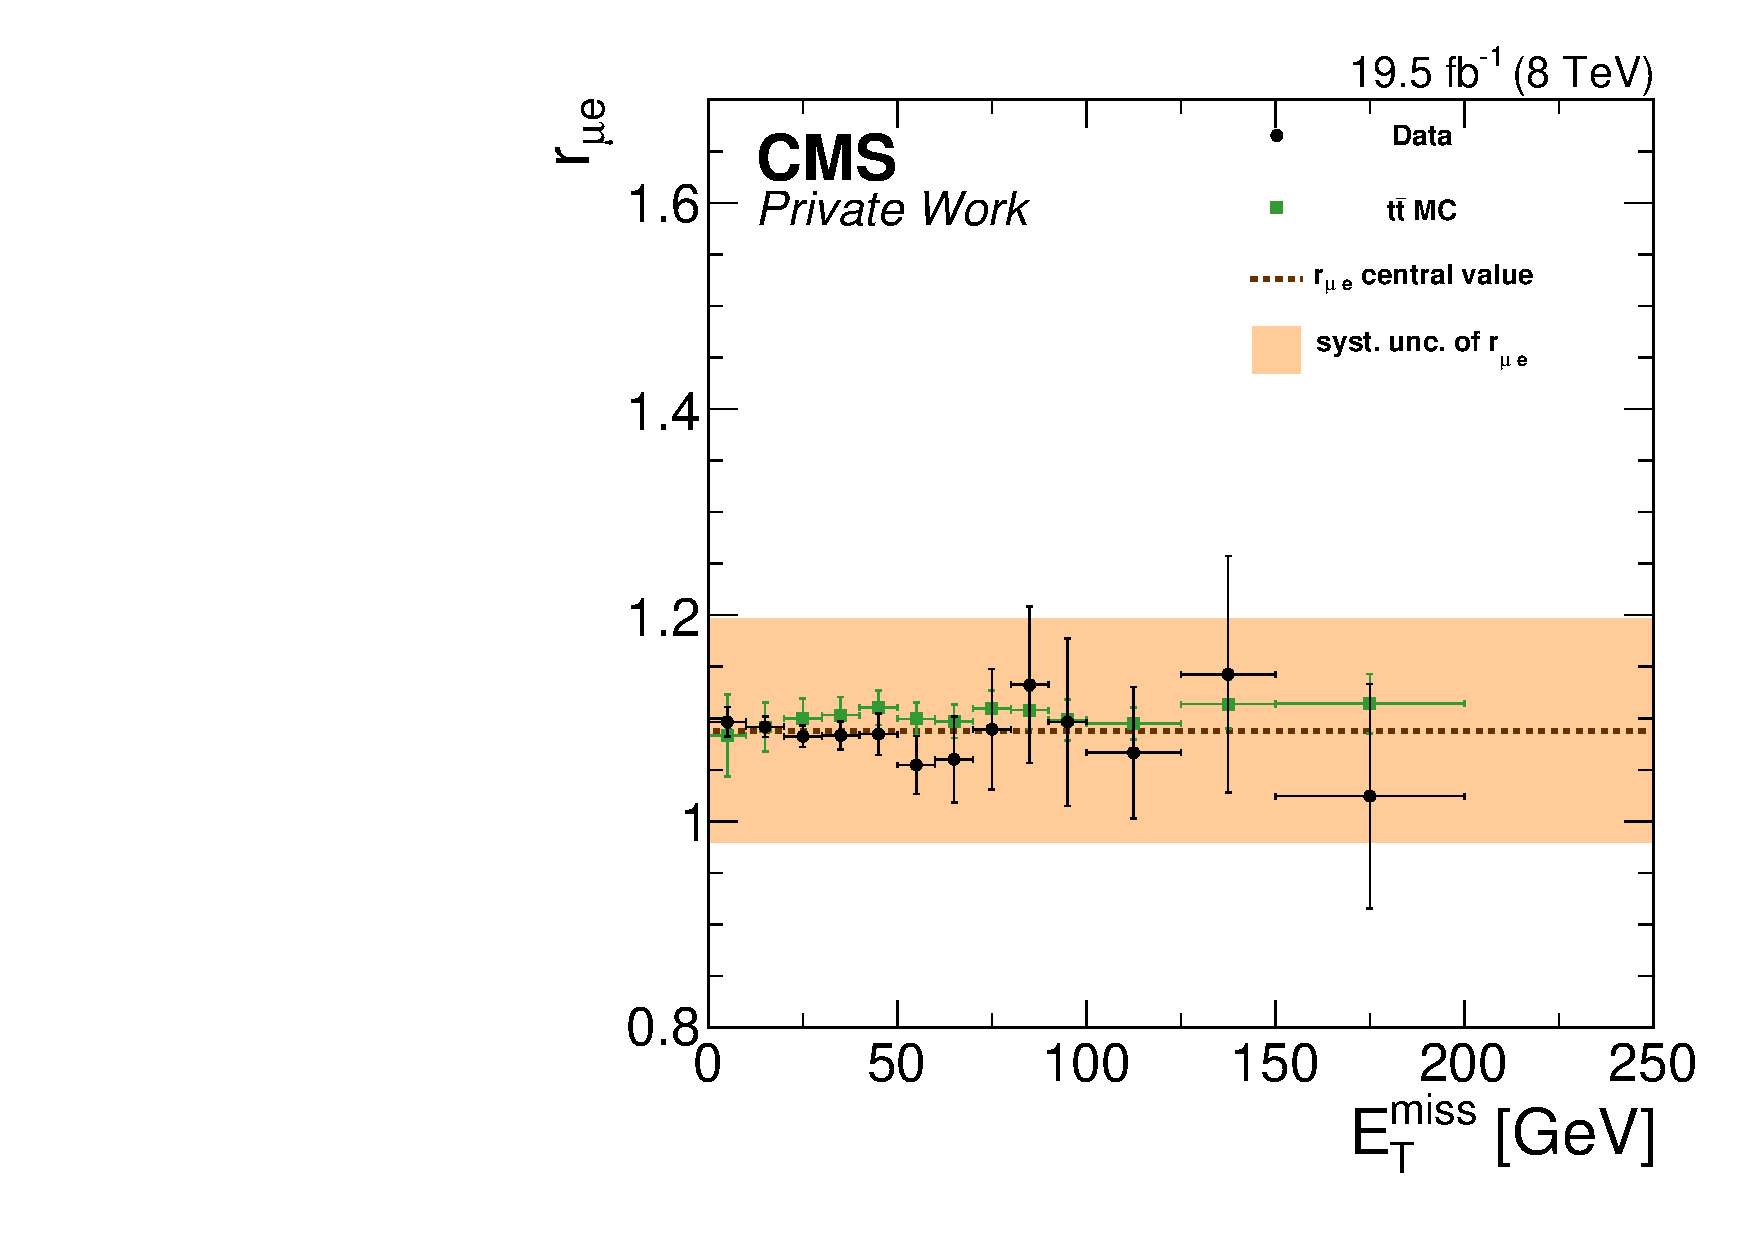
\includegraphics[width=\textwidth]{plots/BG/rmue/rMuE_ZPeakControlCentral_Full2012_MET_None.pdf}
\end{minipage}
\begin{minipage}[t]{0.49\textwidth}
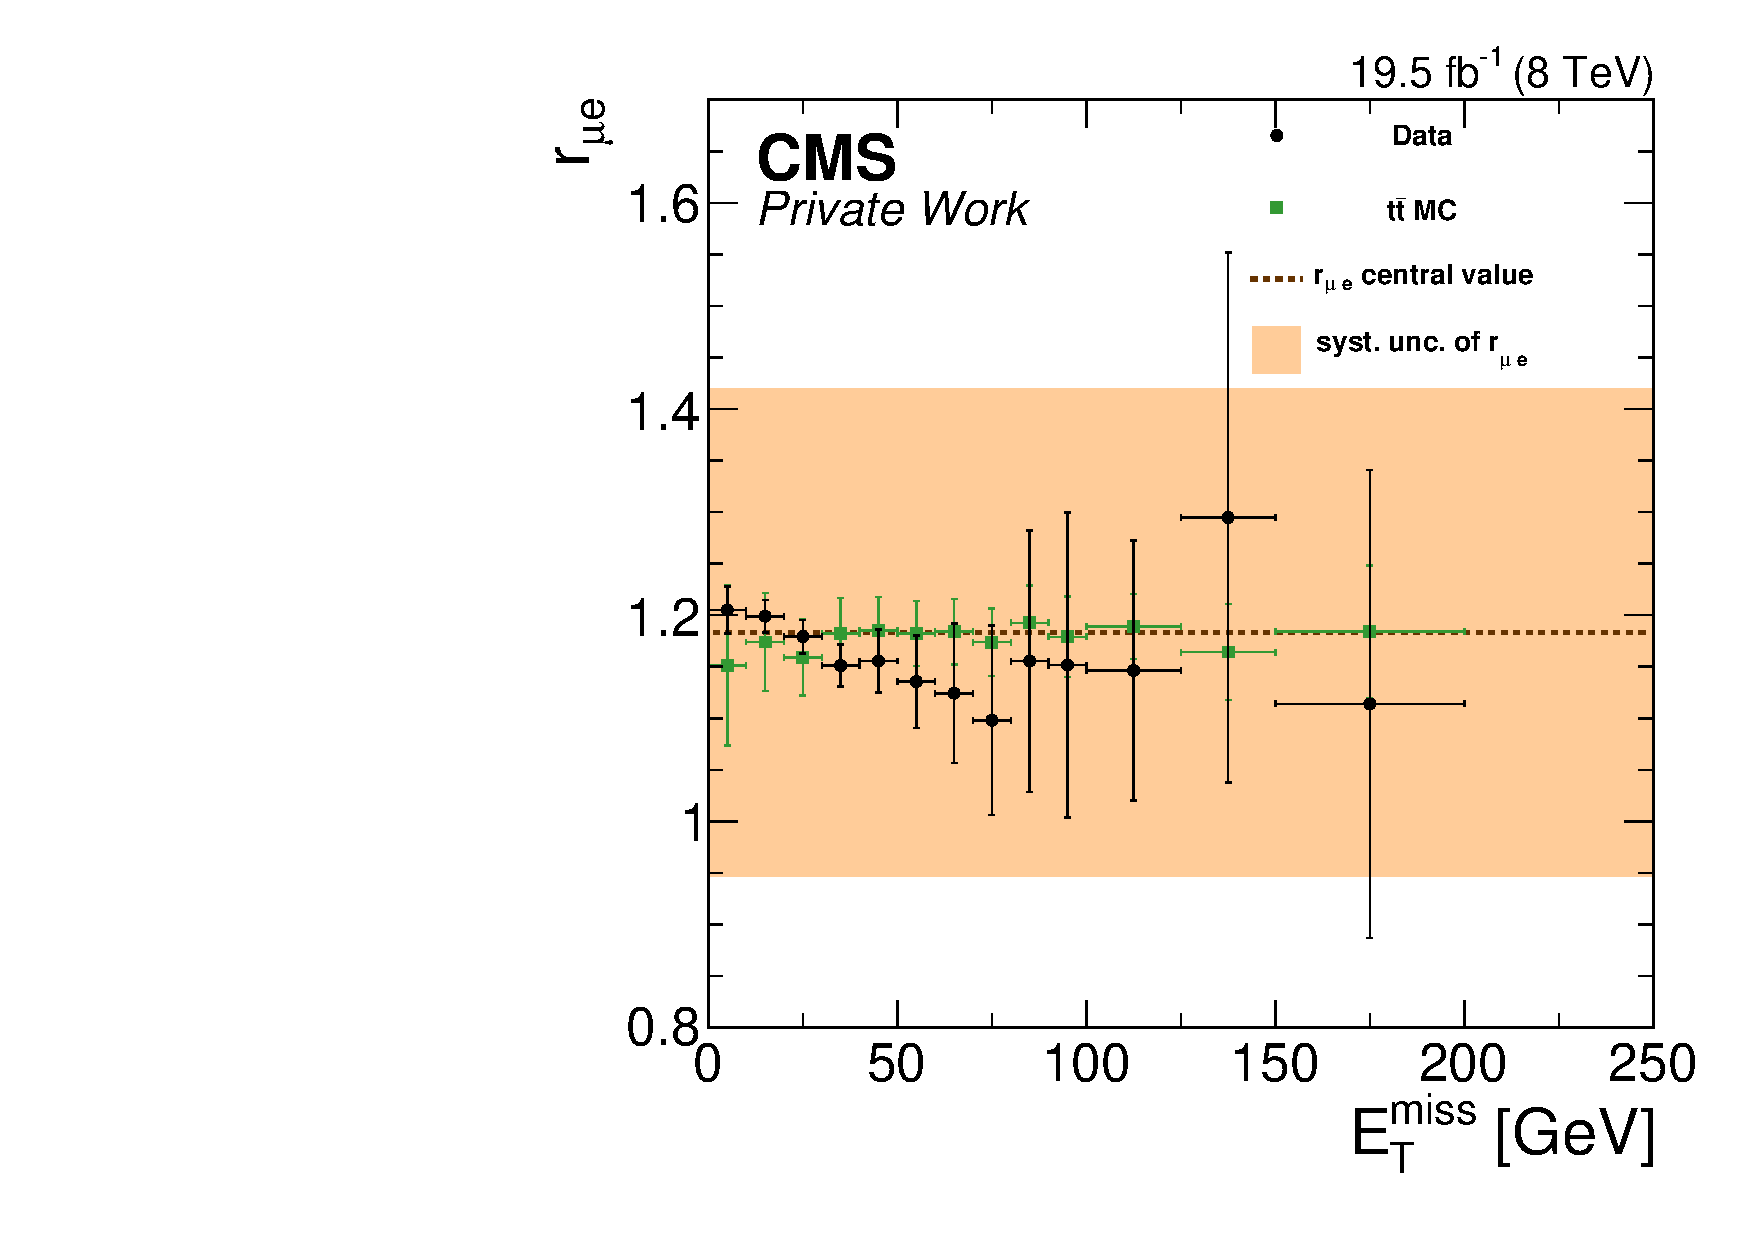
\includegraphics[width=\textwidth]{plots/BG/rmue/rMuE_ZPeakControlForward_Full2012_MET_None.pdf}
\end{minipage}
\begin{minipage}[t]{0.49\textwidth}
  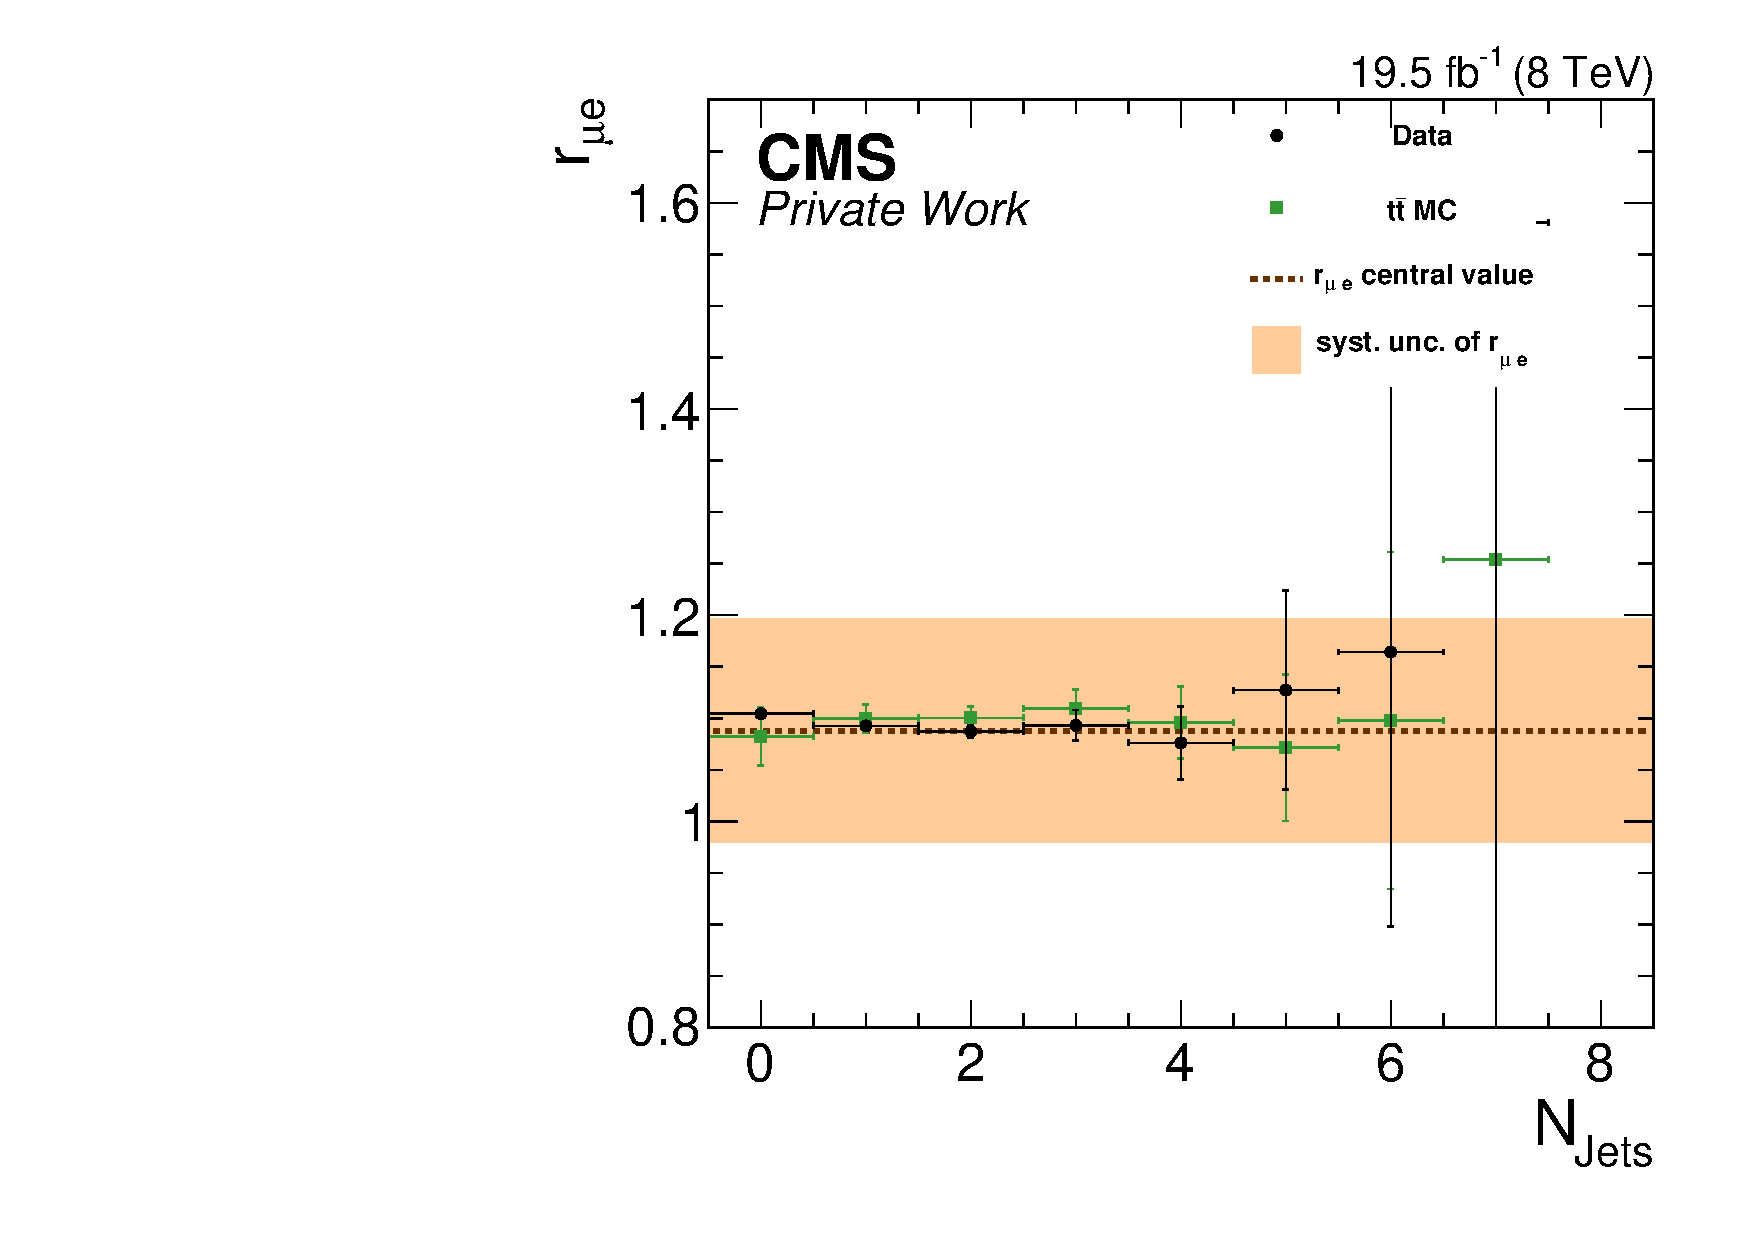
\includegraphics[width=\textwidth]{plots/BG/rmue/rMuE_ZPeakControlCentral_Full2012_NJets_None.pdf}
\end{minipage}
\begin{minipage}[t]{0.49\textwidth}
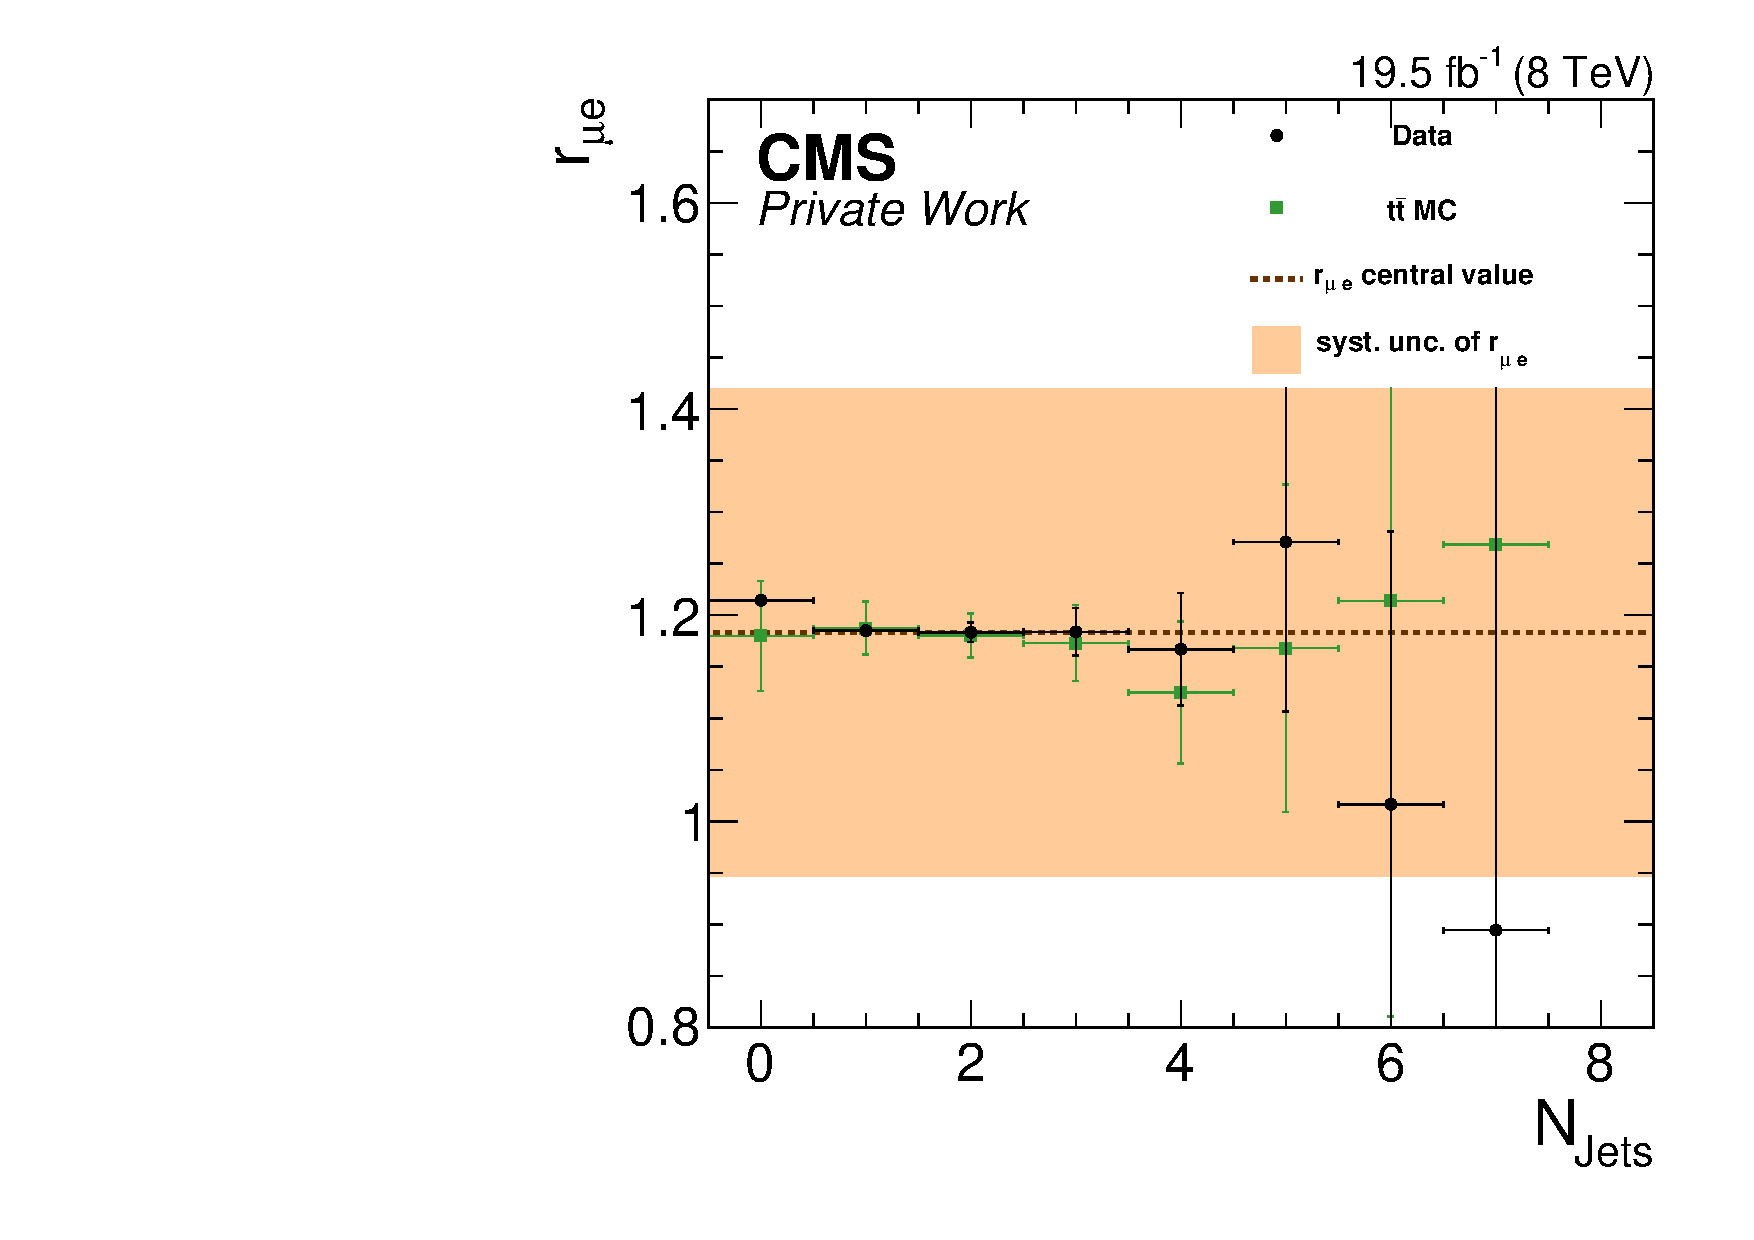
\includegraphics[width=\textwidth]{plots/BG/rmue/rMuE_ZPeakControlForward_Full2012_NJets_None.pdf}
\end{minipage}
\caption{Dependencies of \rmue on \mll (top), \MET (middle), and $N_{jets}$ (bottom) for the central (left) and forward (right) lepton selection. The results on data are shown in black while $t\bar{t}$ simulation is shown in green. The central value is shown as a brown dashed line while the systematic uncertainty is shown as an orange band.}
\label{fig:rmueDependencies}
\end{figure} 
\subsubsection{Measurement of \RT}
\label{sec:triggerEffs}
The trigger efficiencies are measured utilizing an event sample collected with PF $H_T$ triggers. Lepton pairs corresponding to the flavour combination of the trigger in question are selected. To ensure that only correctly reconstructed events are considered in the calculation of the trigger efficiencies, the events are required to have $H_T > \unit{200}{\giga\electronvolt}$, which corresponds to the lowest threshold applied in one of the PF $H_T$ trigger. To ensure that the factorization method is performed on event samples complete orthogonal to the signal region and the $t\bar{t}$ enriched control region, events with $N_{jets} \geq 2$ and $\MET > \unit{100}{\giga\electronvolt}$ are rejected. As the offline lepton selection has more strict requirements compared to the one applied at HLT level, the dilepton trigger should have accepted all these events. The trigger efficiency is therefore defined as the ratio of these event that were accepted by the trigger by the total number of events:
\begin{equation}
\epsilon_{ll}^T = \frac{N_{events}(\text{PF }H_T\text{trigger} \cap \text{dilepton selection} \cap \text{dilepton trigger})}{N_{events}(\text{PF }H_T\text{trigger} \cap \text{dilepton selection})}.
\end{equation}
In the case of \MM and OF events, two triggers are used in the event selection. Therefore their combined efficiency is measured, requesting the logical OR of both. The resulting efficiencies are summarized in Table~\ref{tab:triggerEffs}, separately for the central and forward lepton selection. The trigger efficiencies for \EE and \MM are about 97\% in both the central and forward selection. The efficiency for OF events is lower, about 95\% in the central and 90\% in the forward selection. This shows how the flavour symmetry is broken at trigger level by the \verb+HLT_Mu17_TkMu8+ trigger, which recovers efficiency for the trailing muon leg of the trigger and is not present in the OF triggers.   

\begin{table}[hbp] \caption{Trigger efficiencies measured using \HT baseline trigger. The results are shown for the central and forward regions separately.} 
\centering 
\renewcommand{\arraystretch}{1.2} 
\begin{tabular}{l|c|c|c|c|c|c}     

 & nominator & denominator & $\epsilon_{\ell\ell}^{T} \pm \sigma_{\text{stat}}$ &  nominator & denominator & $\epsilon_{\ell\ell}^{T} \pm \sigma_{\text{stat}}$  \\ 
\hline

&\multicolumn{6}{c}{Data} \\
\hline
&  \multicolumn{3}{c|}{Central } & \multicolumn{3}{c}{ Forward }\\
\hline
ee & 3592 & 3692 & 0.973$\pm$0.003 & 954 & 980 & 0.973$\pm$0.006 \\
$\mu\mu$ & 1375 & 1420 & 0.968$\pm$0.005 & 547 & 566 & 0.966$\pm$0.009 \\
e$\mu$ & 493 & 521 & 0.946$\pm$0.012 & 102 & 114 & 0.895$\pm$0.037 \\
 
 
\hline

& \multicolumn{6}{c}{MC} \\
\hline
&  \multicolumn{3}{c|}{Central } & \multicolumn{3}{c}{ Forward } \\
\hline 
ee & 2912.8 & 2994.6 & 0.973$\pm$0.001 & 943.0 & 969.9 & 0.972$\pm$0.001 \\
$\mu\mu$ & 3241.6 & 3287.9 & 0.986$\pm$0.001 & 1141.6 & 1183.4 & 0.965$\pm$0.001 \\
e$\mu$ & 6279.1 & 6523.1 & 0.963$\pm$0.001 & 2138.8 & 2249.0 & 0.951$\pm$0.001 \\
    
    \hline 
\end{tabular}  
\label{tab:EffValues_Seperated}
\end{table}	

To asses the systematic uncertainties of the trigger efficiency measurement, potential biases due to the choice of the orthogonal trigger  are studied on simulation, using dileptonic $t\bar{t}$ events. On simulation the efficiency can be measured without the requirement of the PF $H_T$ triggers, as no trigger is needed to select the events. The ratio of this true trigger efficiencies to those measured with the PF $H_T$ triggers as a function of \mll is shown in Figure~\ref{fig:triggerEffBias}, separately for SF and OF events. In both cases all deviations from one are in the order of 0.1\% and well compatible with it inside the statistical uncertainties. No bias of the efficiency measurement due to the PF $H_T$ triggers is observed and therefore no systematic uncertainty due to this choice is assigned to the measurement.
\begin{figure}
\begin{center}
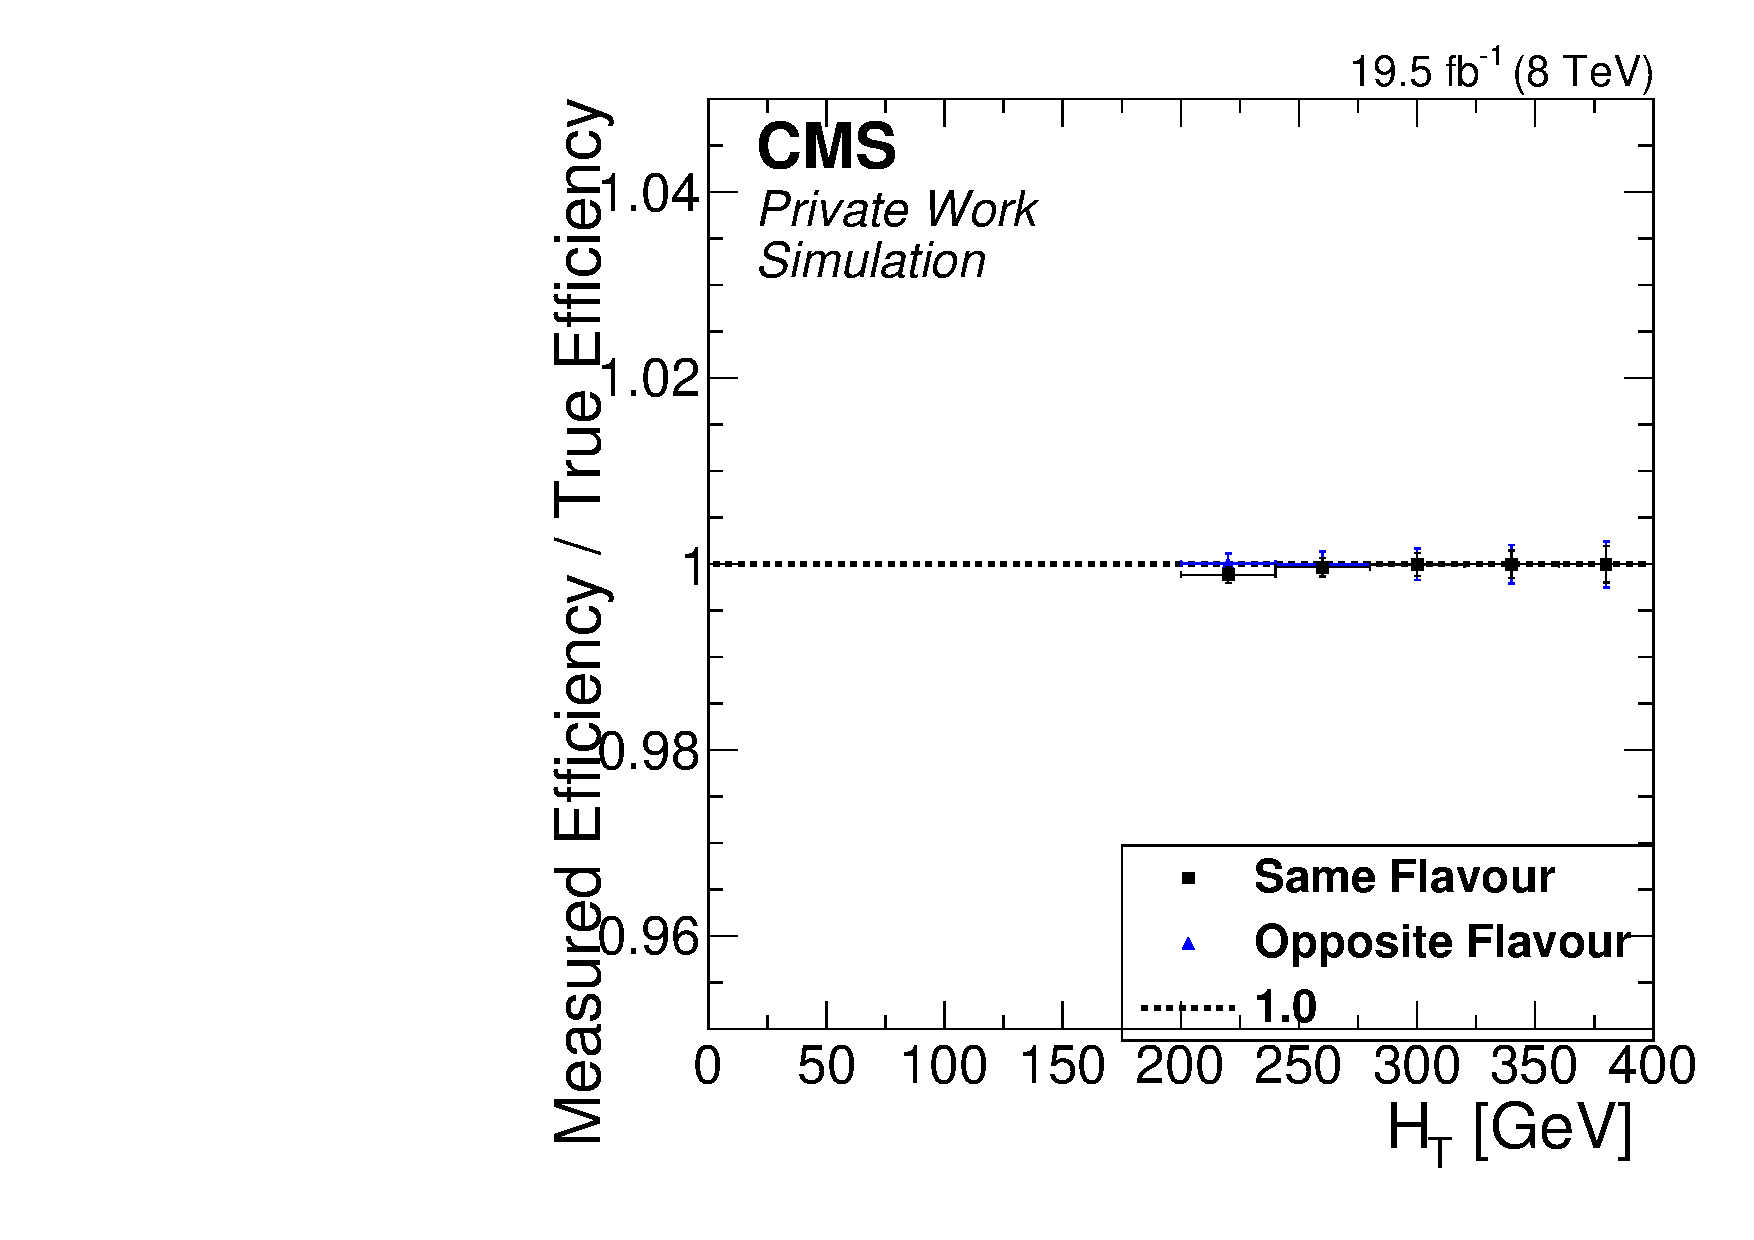
\includegraphics[scale=0.35]{plots/BG/trigger/Triggereff_AlphaTSyst_PFHT_HighHTExclusive_Full2012_HT_None.pdf}
\caption{Ratio of true trigger efficiencies to those calculated using the PF $H_T$ triggers separately for SF and OF events.}
\label{fig:triggerEffBias}
\end{center}
\end{figure}
The turnon of the triggers at low lepton \pt is of particular interest because asymmetries between the lepton flavours are more likely to occur in this difficult environment. The dependence of the trigger efficiency on the \pt of the trailing lepton can be studied using datasets trigger by single lepton triggers. Triggers with \pt thresholds of $\unit{24(27)}{\giga\electronvolt}$ for muons (electrons) are available. These thresholds are relatively low for single lepton triggers, resulting in very strict selection criteria having to be applied on HLT level. Dilepton events are selected in which the leading lepton can be matched  geometrically to the trigger object that fired the single lepton trigger. The trailing lepton is matched to trigger objects that have fired the trailing leg of the dilepton trigger. The efficiency is defined as the number of events in which such a match can be found to the total number of dilepton events. The resulting efficiency curves are shown in Figure~\ref{fig:triggerEffTrailing} for five different trailing lepton trigger legs and combining the central and forward selection. It can be seen that the efficiency for trailing electrons are virtually the same for the dielectron and OF triggers (black and light blue markers). The same is true for trailing muons in the dimuon and OF triggers (brown and dark blue markers). However, the efficiency for trailing muons in the \verb+HLT_Mu17_TkMu8+ trigger is significantly higher than those in the trigger paths not using the tracker information, as expected. Trailing muons have a much sharper turnon than trailing electrons, being fully efficient already at a \pt of $\unit{10}{\giga\electronvolt}$. For electrons the plateau is reached only above $\unit{\approx 30}{\giga\electronvolt}$. The turnon is steeper for trailing electrons in the dielectron trigger compared to those in the OF trigger, resulting in an increased deviation from flavour symmetry below $\unit{20}{\giga\electronvolt}$. As in the design of the analysis the precision and stability of the background prediction was given priority over lepton acceptance, events with trailing leptons in this \pt range are rejected.  
\begin{figure}
\begin{center}
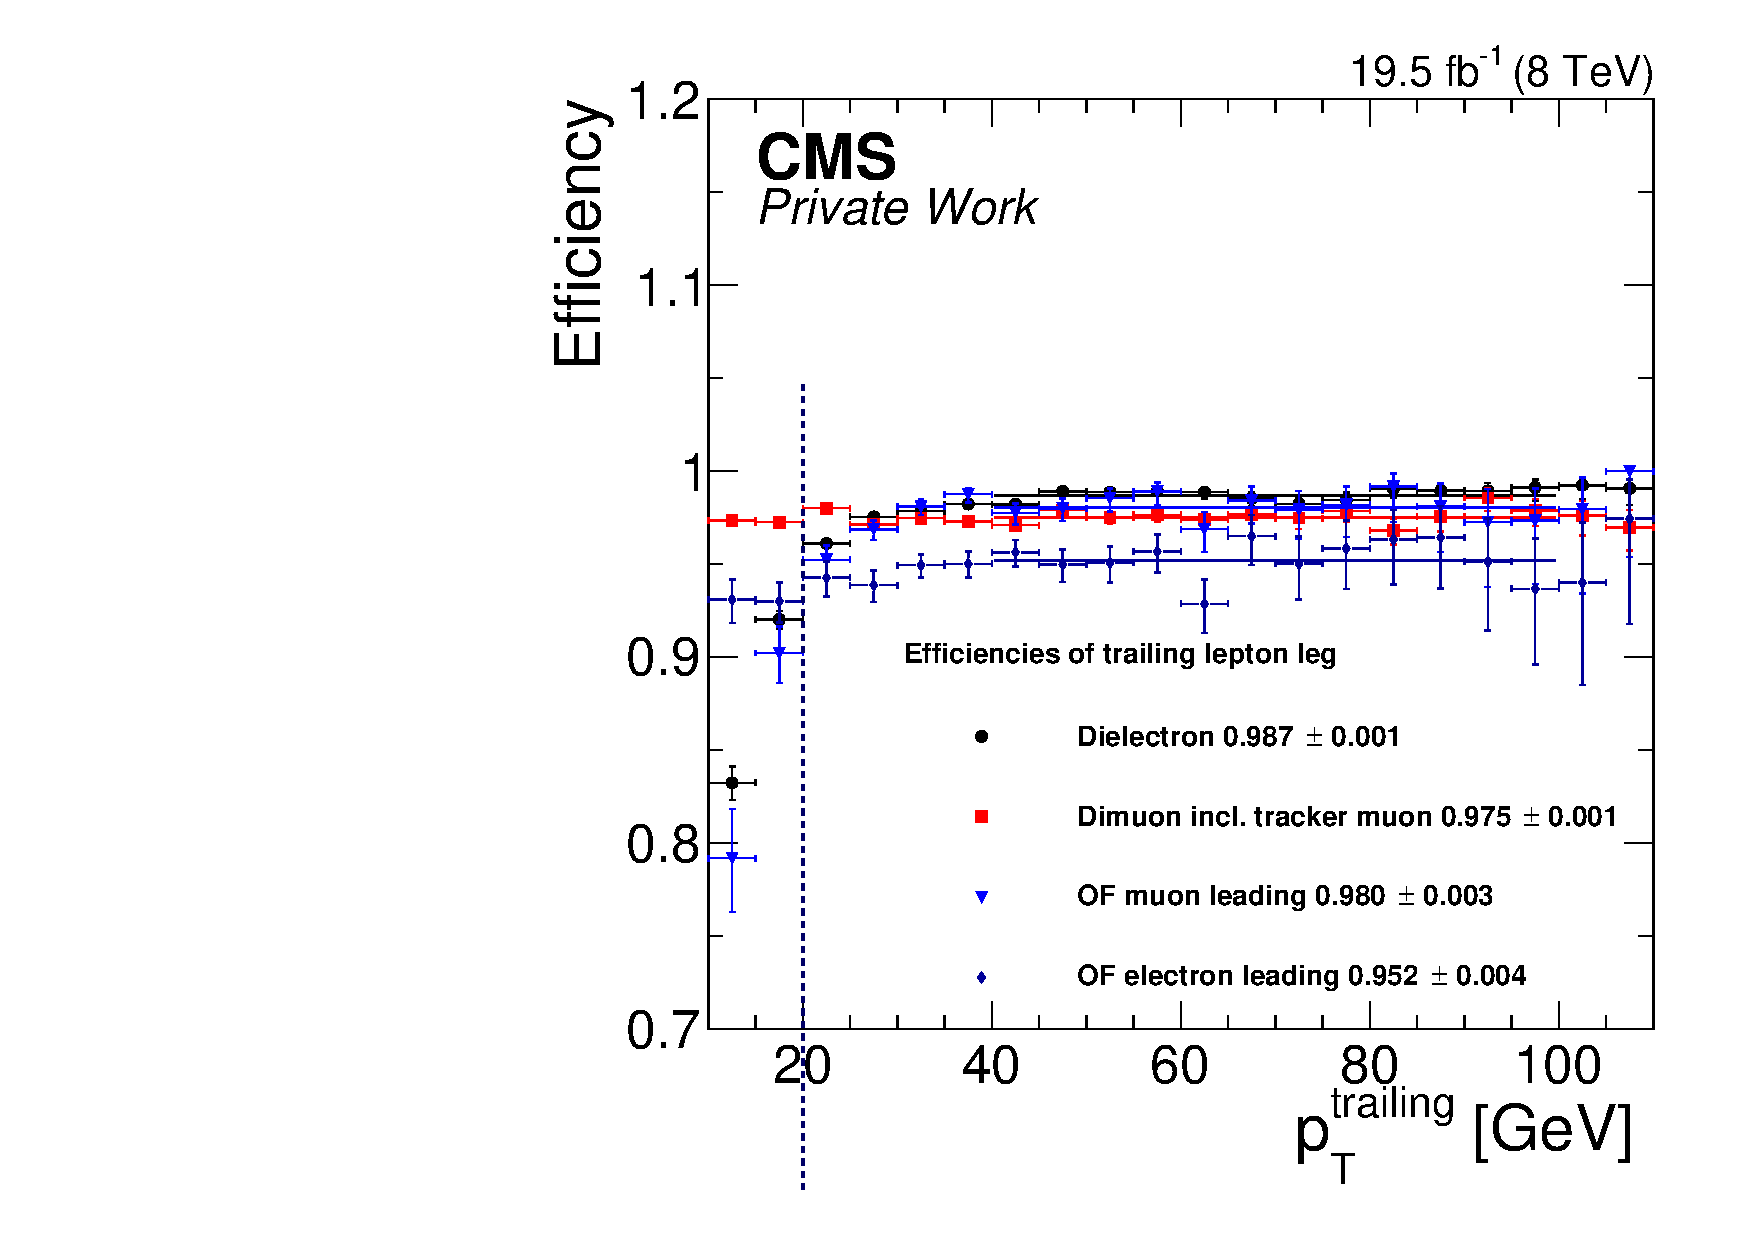
\includegraphics[scale=0.35]{plots/BG/trigger/Triggereff_SingleLepton_HighHTExclusive_Full2012_TrailingPt_leadingPt30Single.pdf}
\caption{Ratio of true trigger efficiencies to those calculated using the PF $H_T$ triggers separately for SF and OF events.}
\label{fig:triggerEffTrailing}
\end{center}
\end{figure} 
To asses the systematic uncertainties of the trigger efficiency measurement, the dependency of $R_T$ as used in the calculation of \Rsfof on different observables is tested. Here a dataset not triggered by $\alpha_T$ triggers is used, as the PF $H_T$ triggers do not provide enough events for these studies. A 5\% systematic uncertainty is assigned to each trigger efficiency, resulting in an uncertainty of 6.4\% on $R_T$, covering all observed deviations from the the measured value of $R_T$ within the statistical uncertainties, as shown in Figure\ref{fig:RTDependencies}. Studies of further variables can be found in Appendix~\ref{app:RT}
\begin{figure}[htbp]
\centering
\begin{minipage}[t]{0.49\textwidth}
  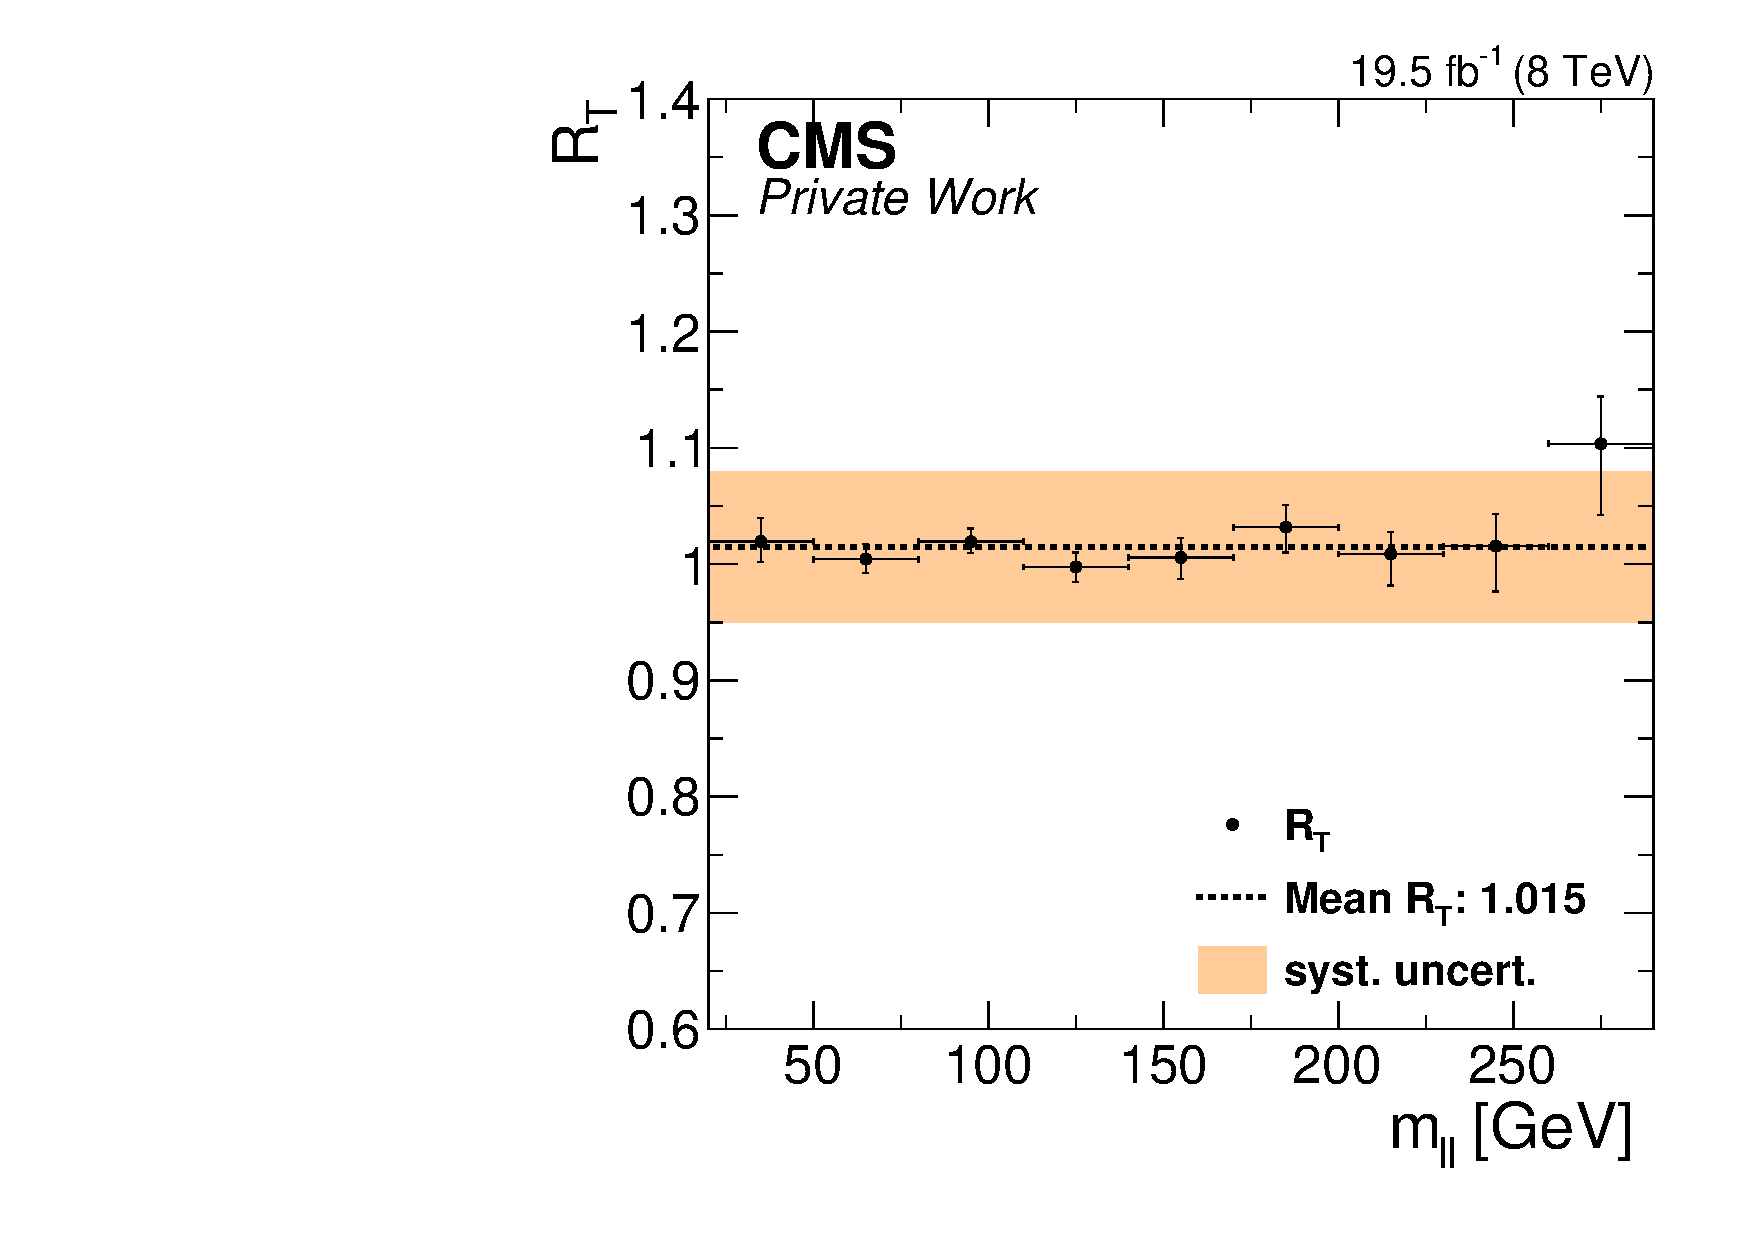
\includegraphics[width=\textwidth]{plots/BG/trigger/Triggereff_SFvsOF_Syst_AlphaT_HighHTExclusiveCentral_Full2012_Mll_None.pdf}
\end{minipage}
\begin{minipage}[t]{0.49\textwidth}
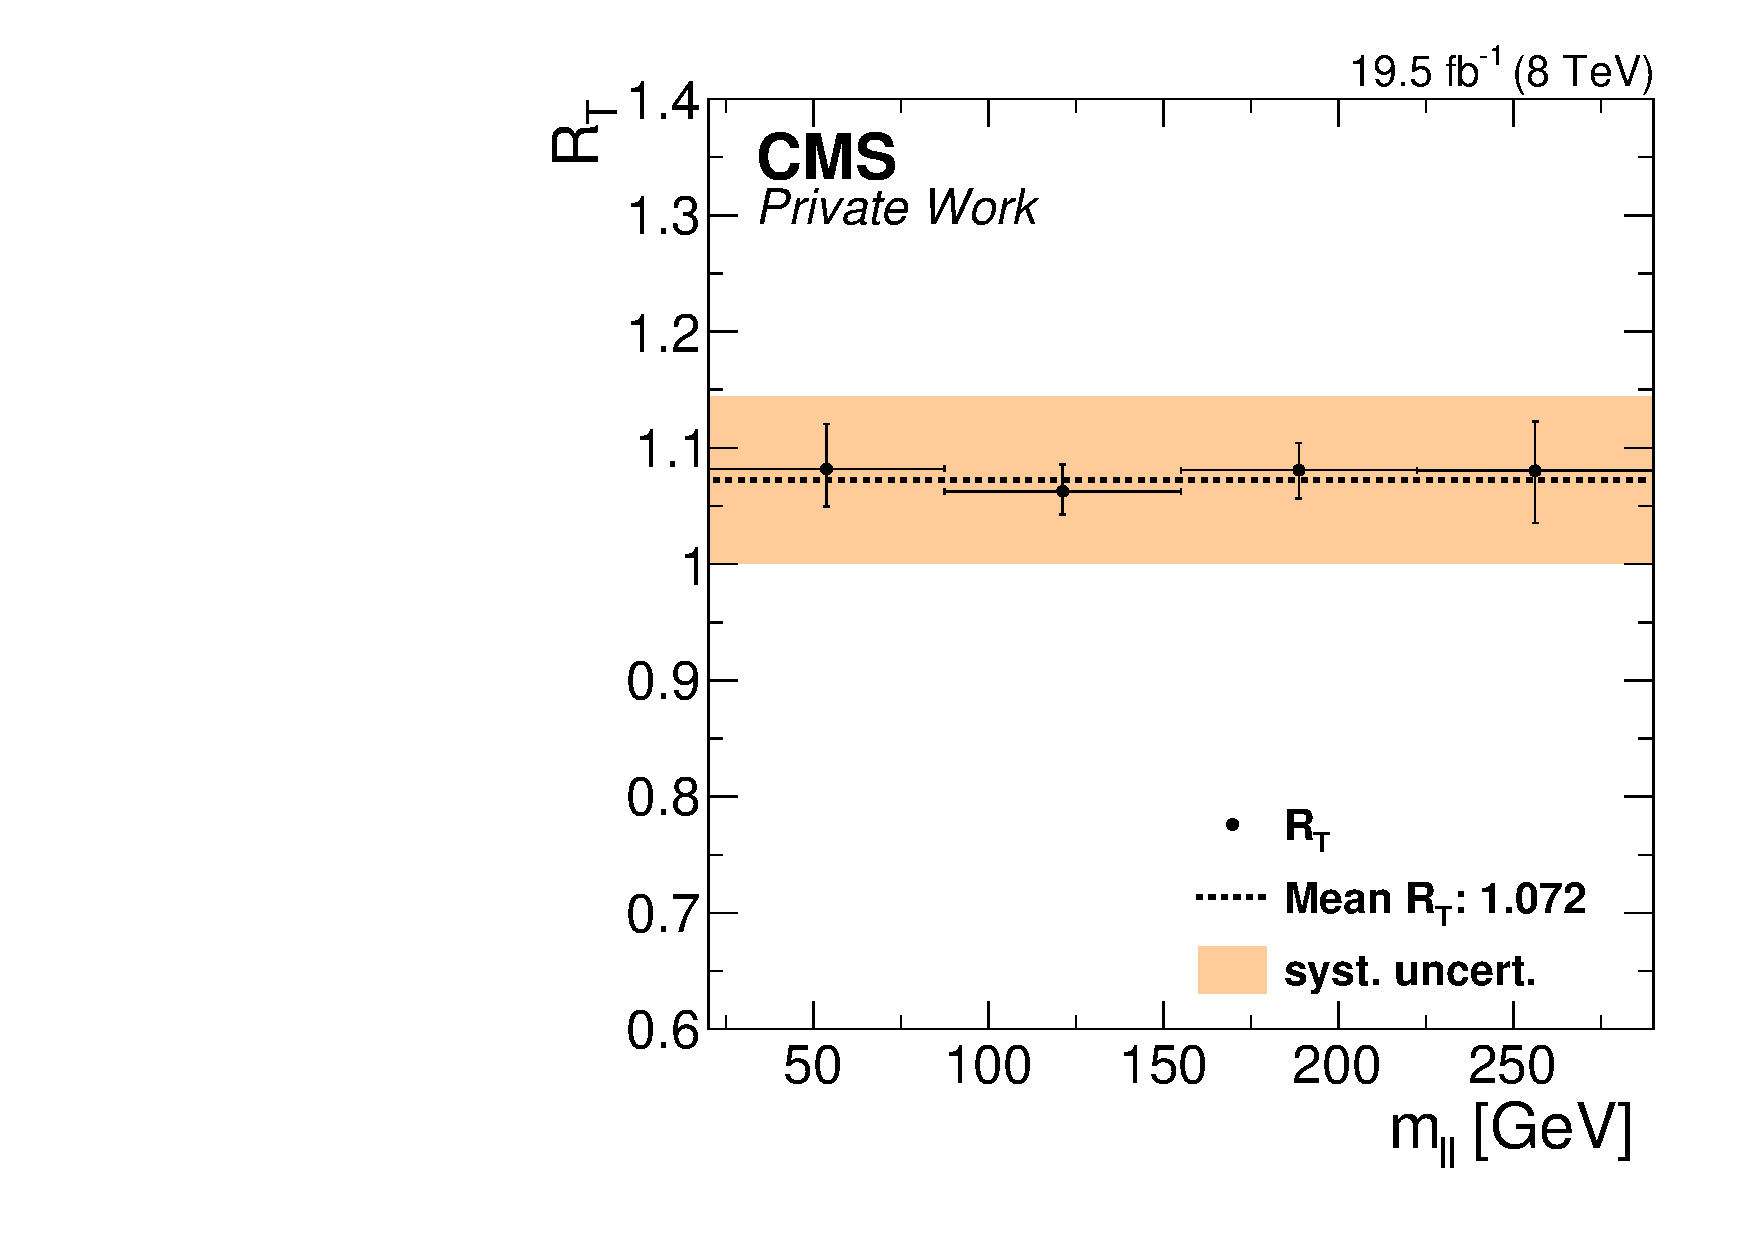
\includegraphics[width=\textwidth]{plots/BG/trigger/Triggereff_SFvsOF_Syst_AlphaT_HighHTExclusiveForward_Full2012_Mll_None.pdf}
\end{minipage}
\begin{minipage}[t]{0.49\textwidth}
  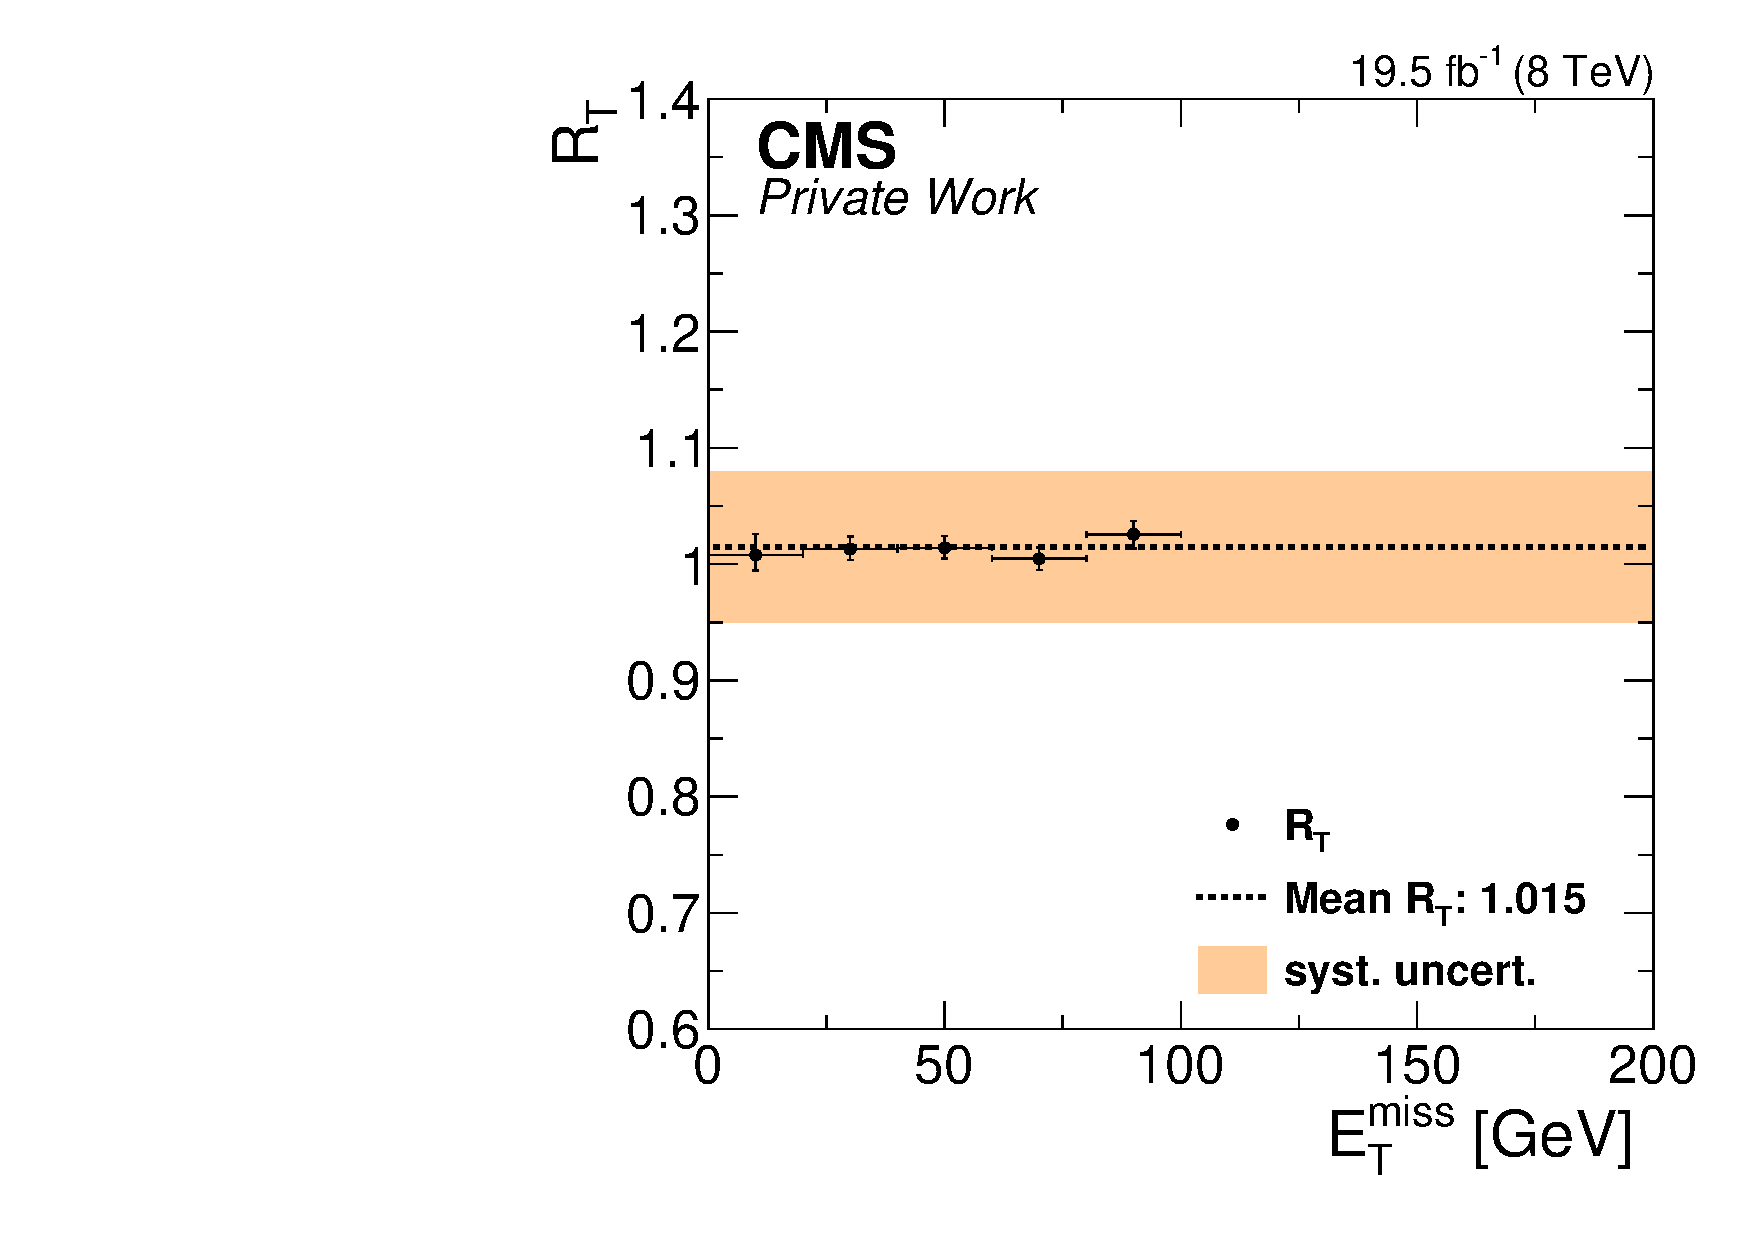
\includegraphics[width=\textwidth]{plots/BG/trigger/Triggereff_SFvsOF_Syst_AlphaT_HighHTExclusiveCentral_Full2012_MET_None.pdf}
\end{minipage}
\begin{minipage}[t]{0.49\textwidth}
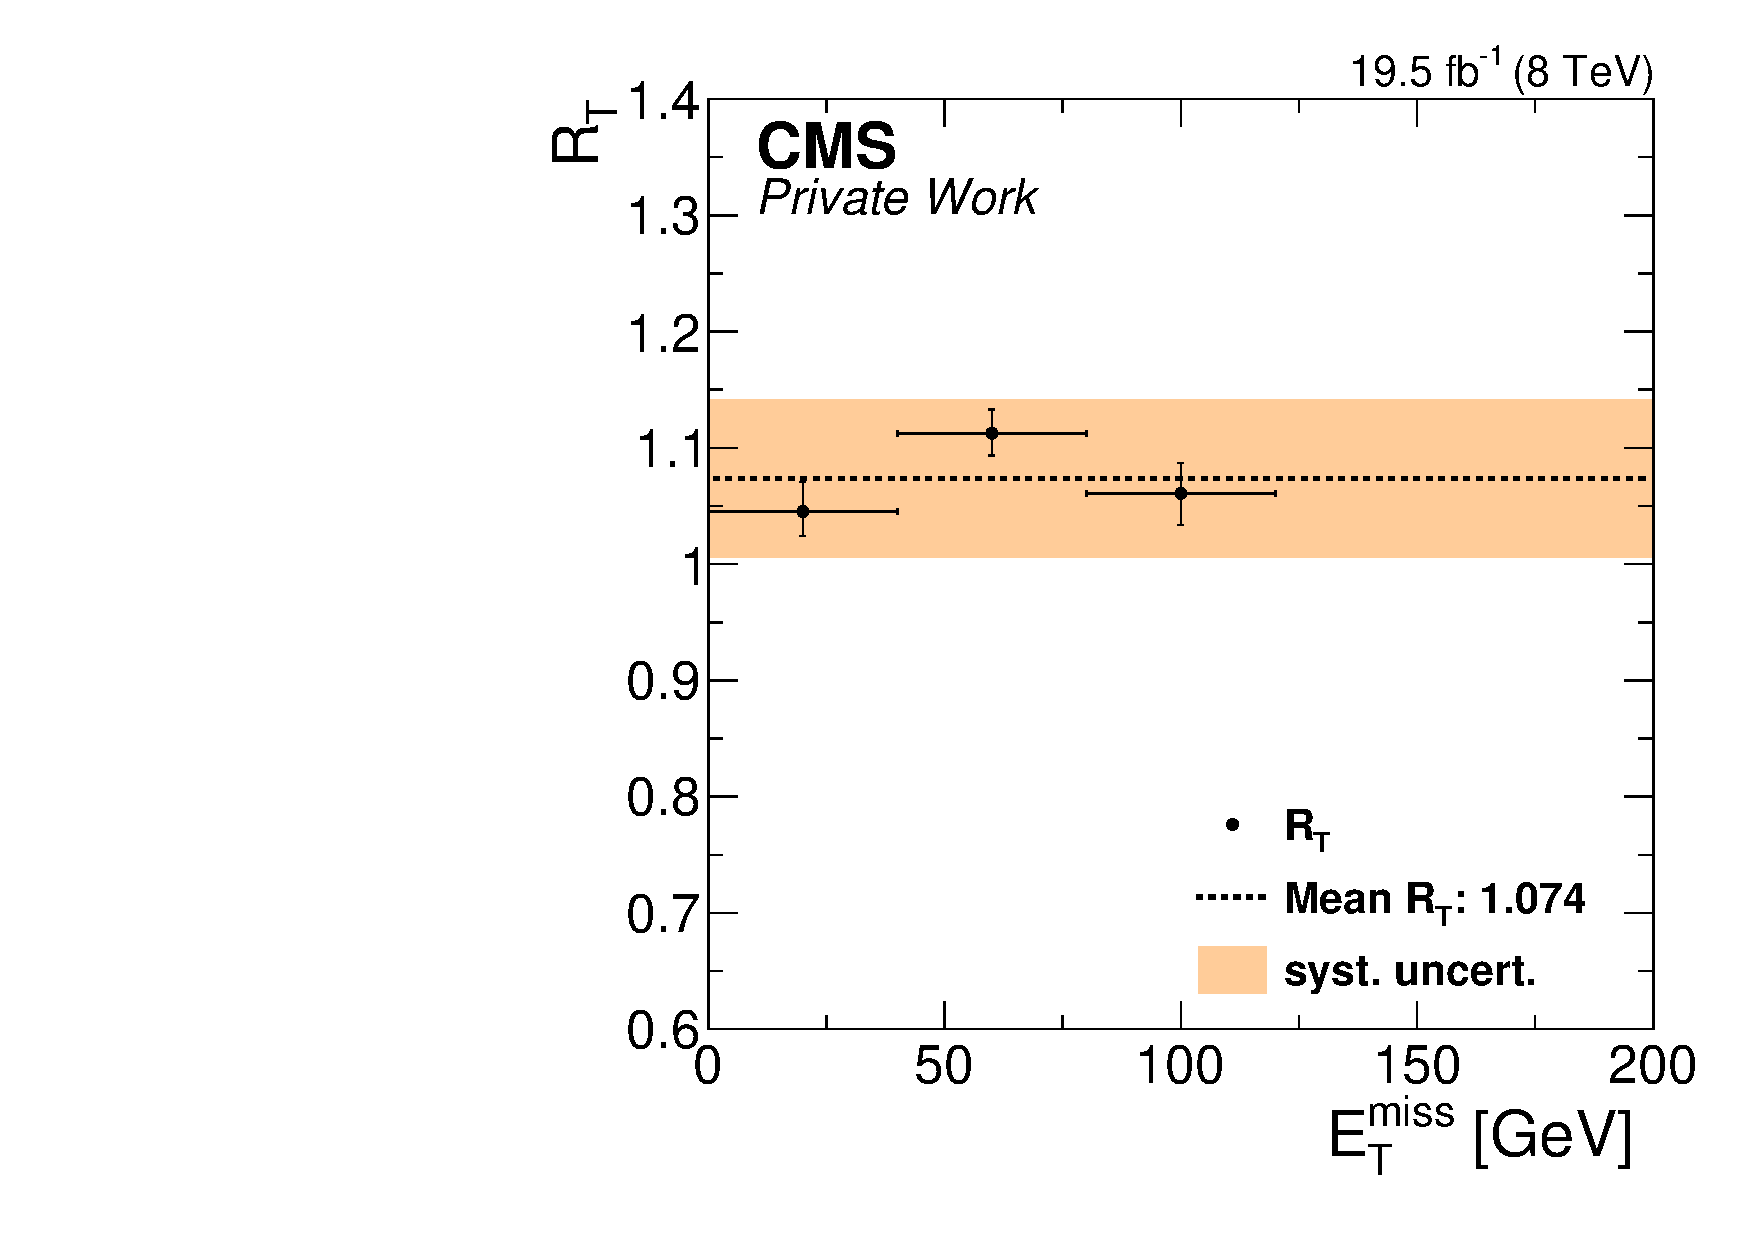
\includegraphics[width=\textwidth]{plots/BG/trigger/Triggereff_SFvsOF_Syst_AlphaT_HighHTExclusiveForward_Full2012_MET_None.pdf}
\end{minipage}
\begin{minipage}[t]{0.49\textwidth}
  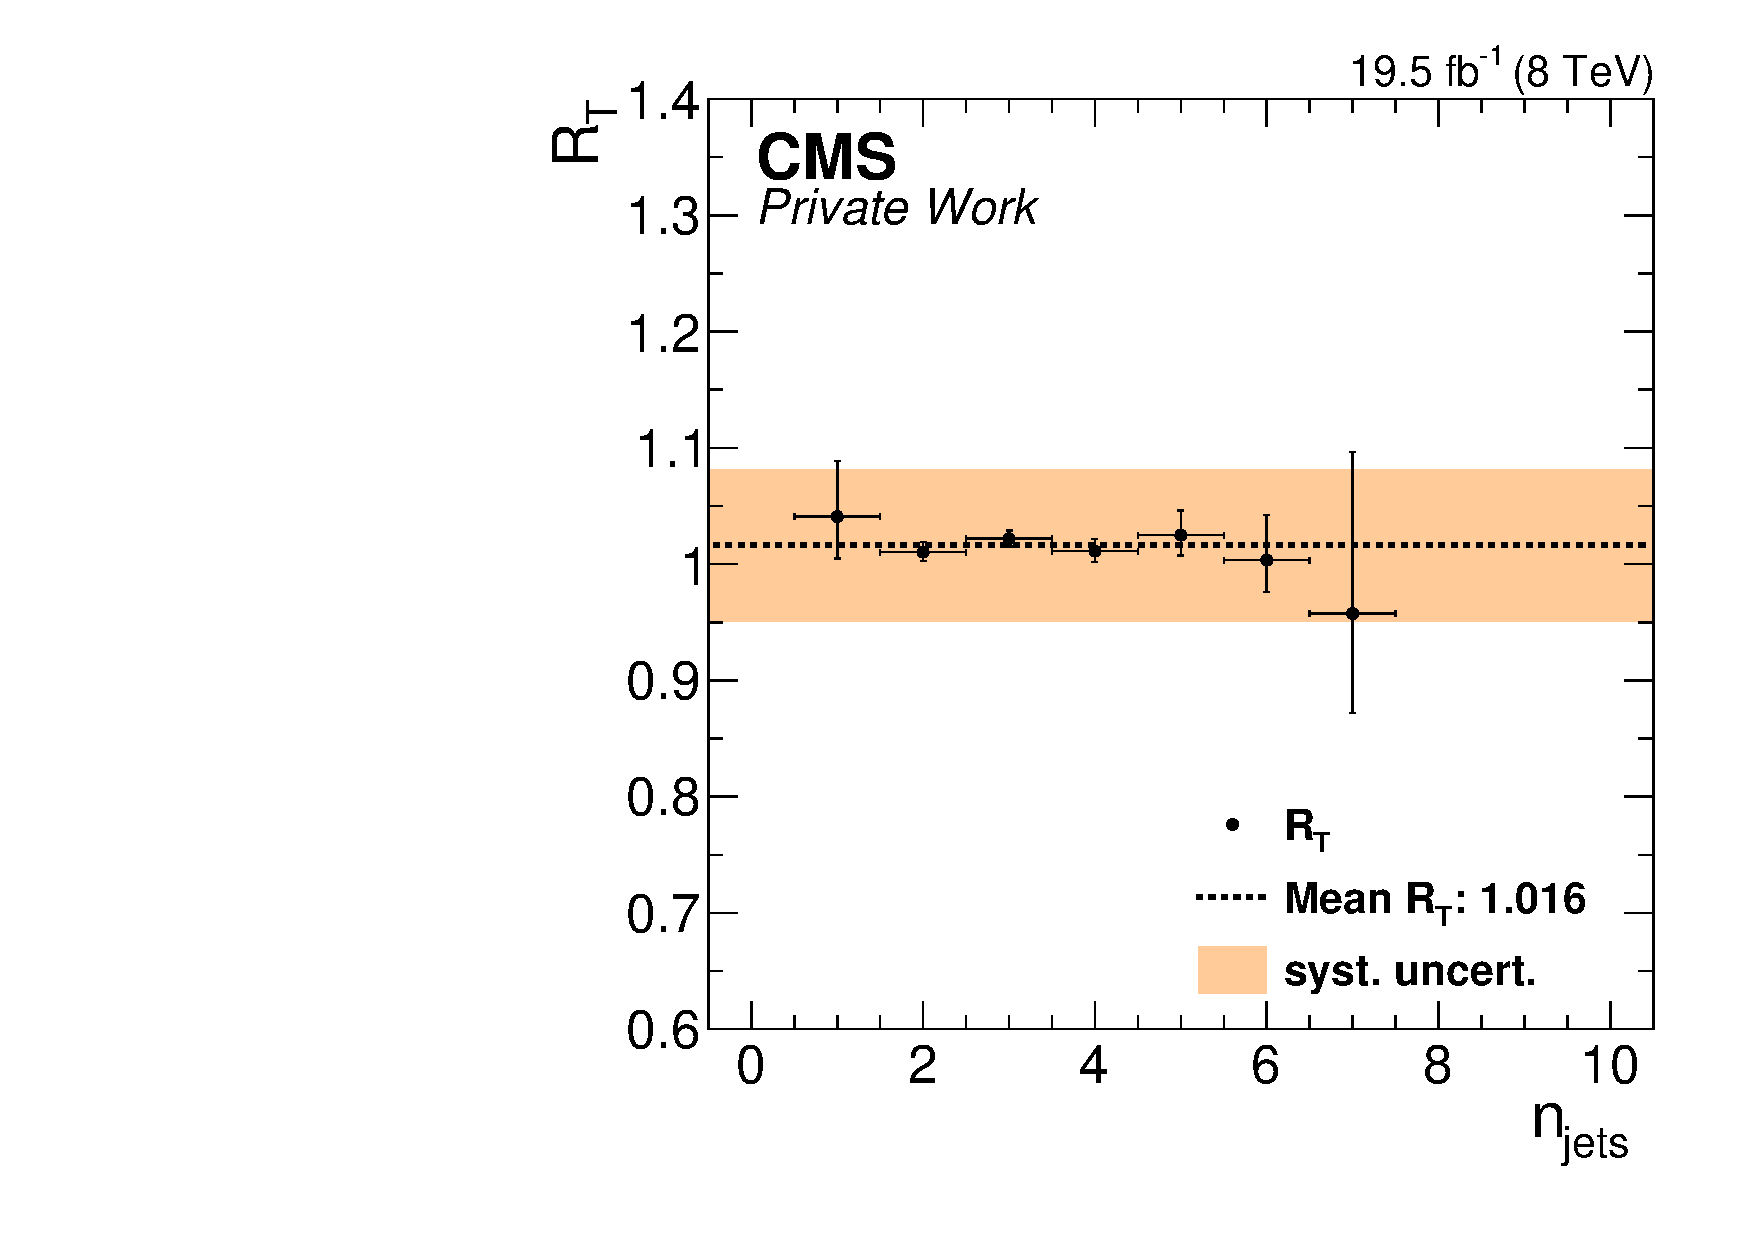
\includegraphics[width=\textwidth]{plots/BG/trigger/Triggereff_SFvsOF_Syst_AlphaT_HighHTExclusiveCentral_Full2012_NJets_None.pdf}
\end{minipage}
\begin{minipage}[t]{0.49\textwidth}
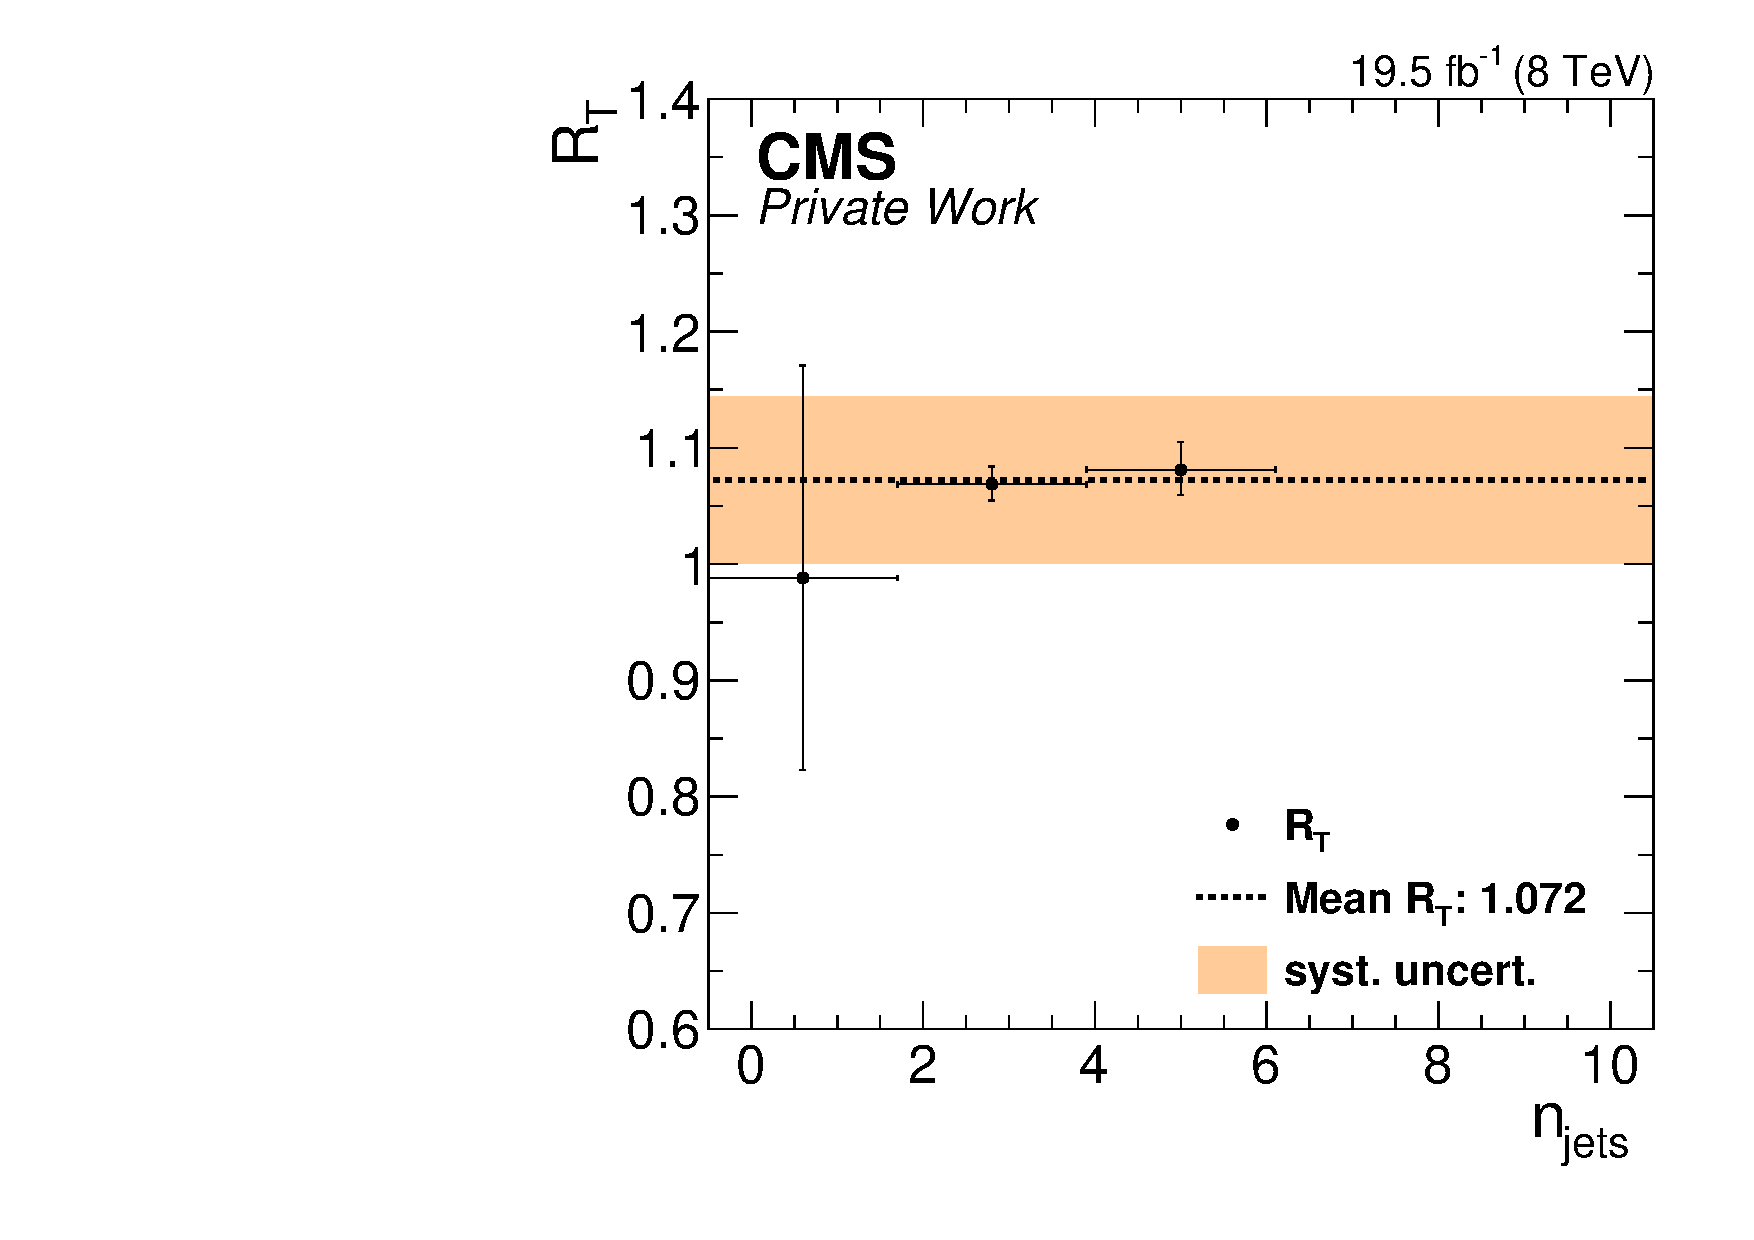
\includegraphics[width=\textwidth]{plots/BG/trigger/Triggereff_SFvsOF_Syst_AlphaT_HighHTExclusiveForward_Full2012_NJets_None.pdf}
\end{minipage}
\caption{Dependencies of $R_T$ on \mll (top), \MET (middle), and $N_{jets}$ (bottom) for the central (left) and forward (right) lepton selection. The results on data are shown in black. The central value is shown as a black dashed line while the systematic uncertainty is shown as an orange band.}
\label{fig:RTDependencies}
\end{figure} 
\subsubsection{Results of the factorization method}
The results of the factorization methods are summarized in Table~\ref{tab:factorization}. The factor $R_T$ is calculated from the trigger efficiencies in Table~\ref{tab:EffValues_Seperated} as $R_T = \sqrt{\frac{\epsilon_{ee}^{T}\cdot\epsilon_{\mu\mu}^{T} }{\epsilon_{e\mu}^{T}}}$. The resulting correction factors \Rsfof, \Reeof, and \Rmmof are calculated as described in equations~\ref{eq:nee}-\ref{eq:nsf}.  

\begin{table}[hbtp]
 \renewcommand{\arraystretch}{1.3}
 \setlength{\belowcaptionskip}{6pt}
 \centering
 \caption{Result of the determination of \Rsfof, \Reeof, and \Rmmof using the factorisation method.}
  \label{tab:factorisation}
  \begin{tabular}{l| c c| c c }

    & \multicolumn{2}{c}{Central} & \multicolumn{2}{c}{Forward} \\ 
    								
    \hline
    & Data & MC & Data & MC \\ 
 
    \hline
        \rmue       &  1.088$\pm$0.109  &  1.103$\pm$0.110      &  1.183$\pm$0.237 &   1.207$\pm$0.241    \\
        $R_{T}$       &  1.026$\pm$0.066  &  1.017$\pm$0.065      &  1.084$\pm$0.079 &   1.018$\pm$0.069    \\

\hline
\hline
        \Rsfof       &  1.029$\pm$0.067  &  1.031$\pm$0.067      &  1.099$\pm$0.088 &   1.103$\pm$0.091    \\
        \Reeof       &  0.471$\pm$0.116  &  0.465$\pm$0.117      &  0.458$\pm$0.259 &   0.449$\pm$0.264    \\
        \Rmmof       &  0.558$\pm$0.117  &  0.565$\pm$0.119      &  0.641$\pm$0.261 &   0.654$\pm$0.266    \\

  \end{tabular}
\end{table}



As for the direct measurements in the control region, the observed deviations of \Rsfof from one are small and inside the uncertainties of the method. Because the uncertainty on \rmue cancels out to a large degree in the calculation \Rsfof, the total uncertainty is dominated by the uncertainty on $R_T$, while for \Reeof and \Rmmof the uncertainty of \rmue is the dominant one. This results in much larger uncertainties on the latter two factors. The dependency of \Rsfof on \rmue and $R_T$ is illustrated in Figure~\ref{fig:rmuePropaganda}. The measured values of \rmue and \Rsfof are shown as straight lines, surrounded by bands indicating their uncertainties. The red line shows the value of \Rsfof corresponding to a given \rmue, under the assumption that the trigger efficiencies stay constant. It can be seen that 


\begin{figure}[htbp]
\centering
\begin{minipage}[t]{0.49\textwidth}
  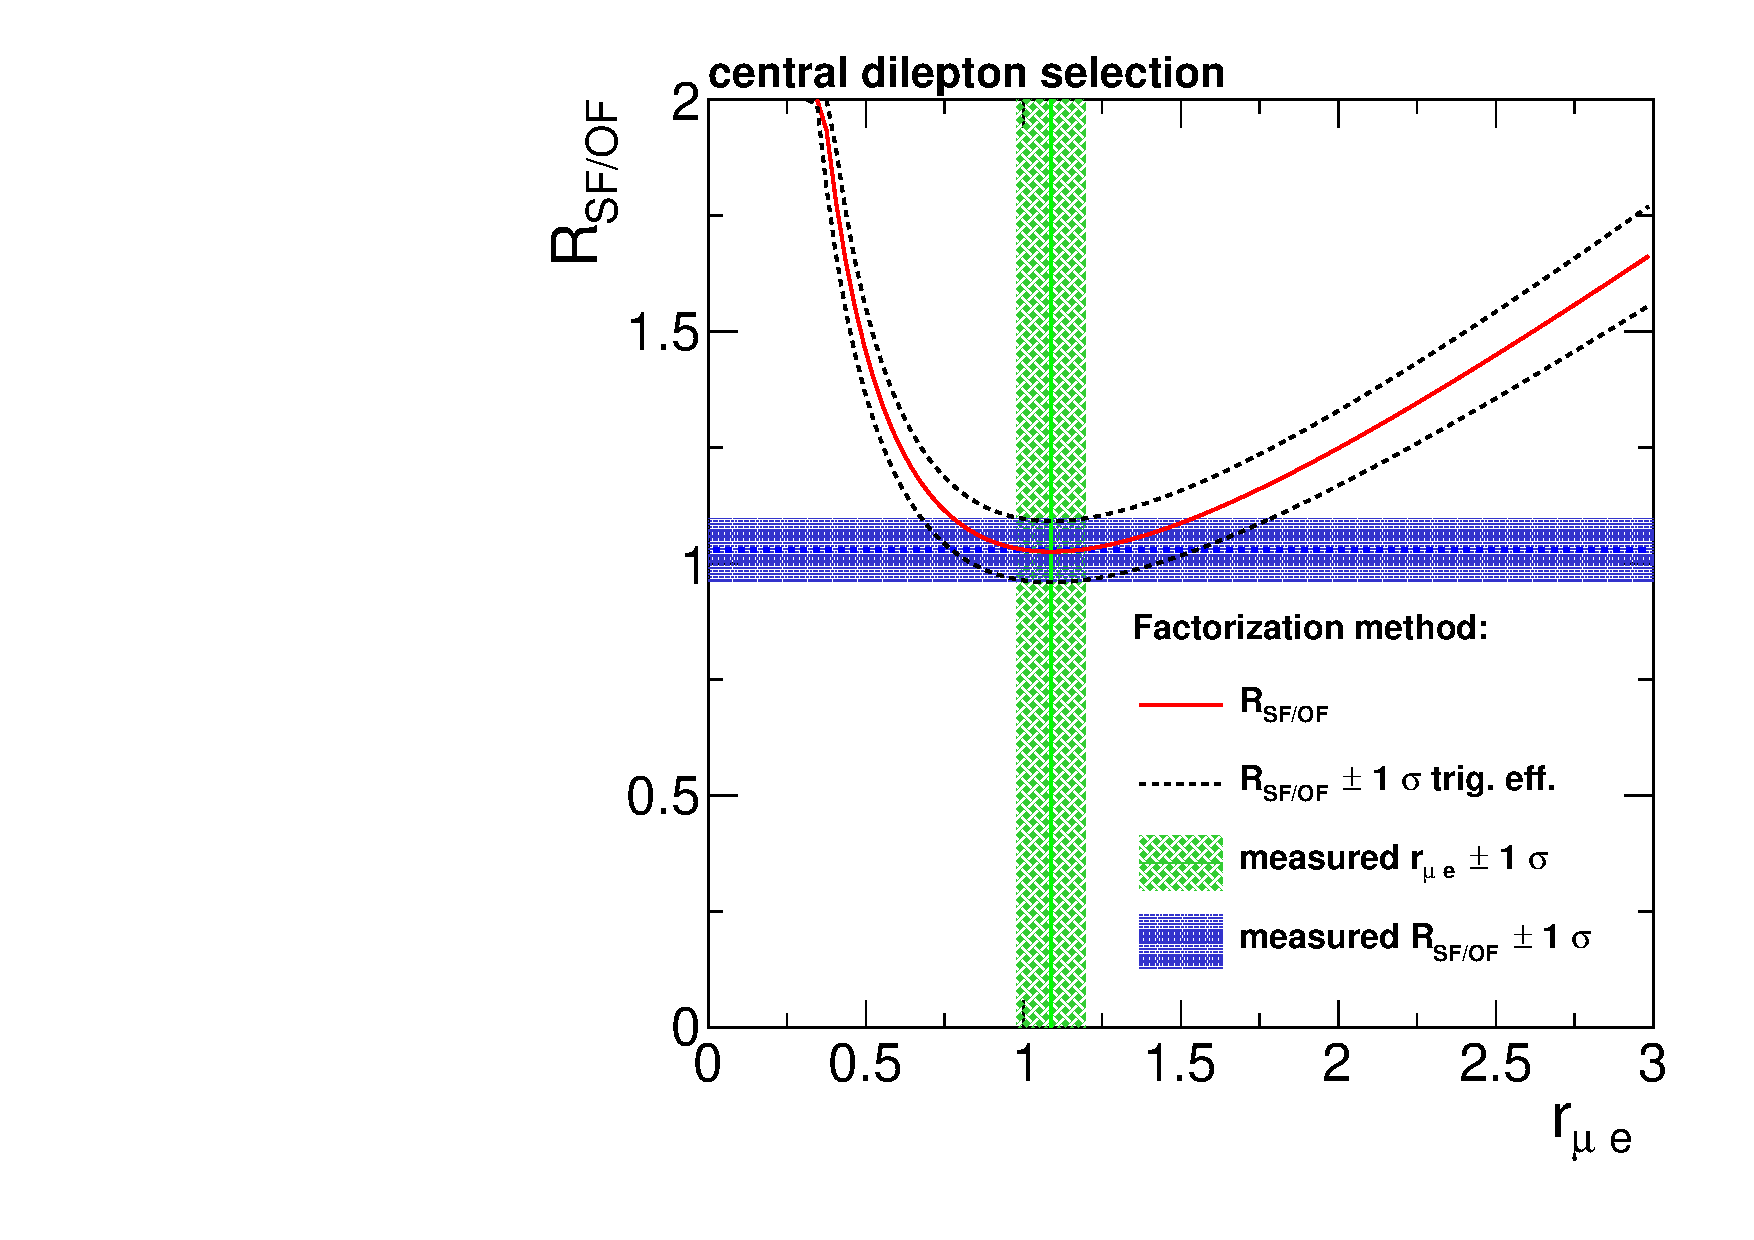
\includegraphics[width=\textwidth]{plots/BG/rmue/rMuEPropaganda_central.pdf}
\end{minipage}
\begin{minipage}[t]{0.49\textwidth}
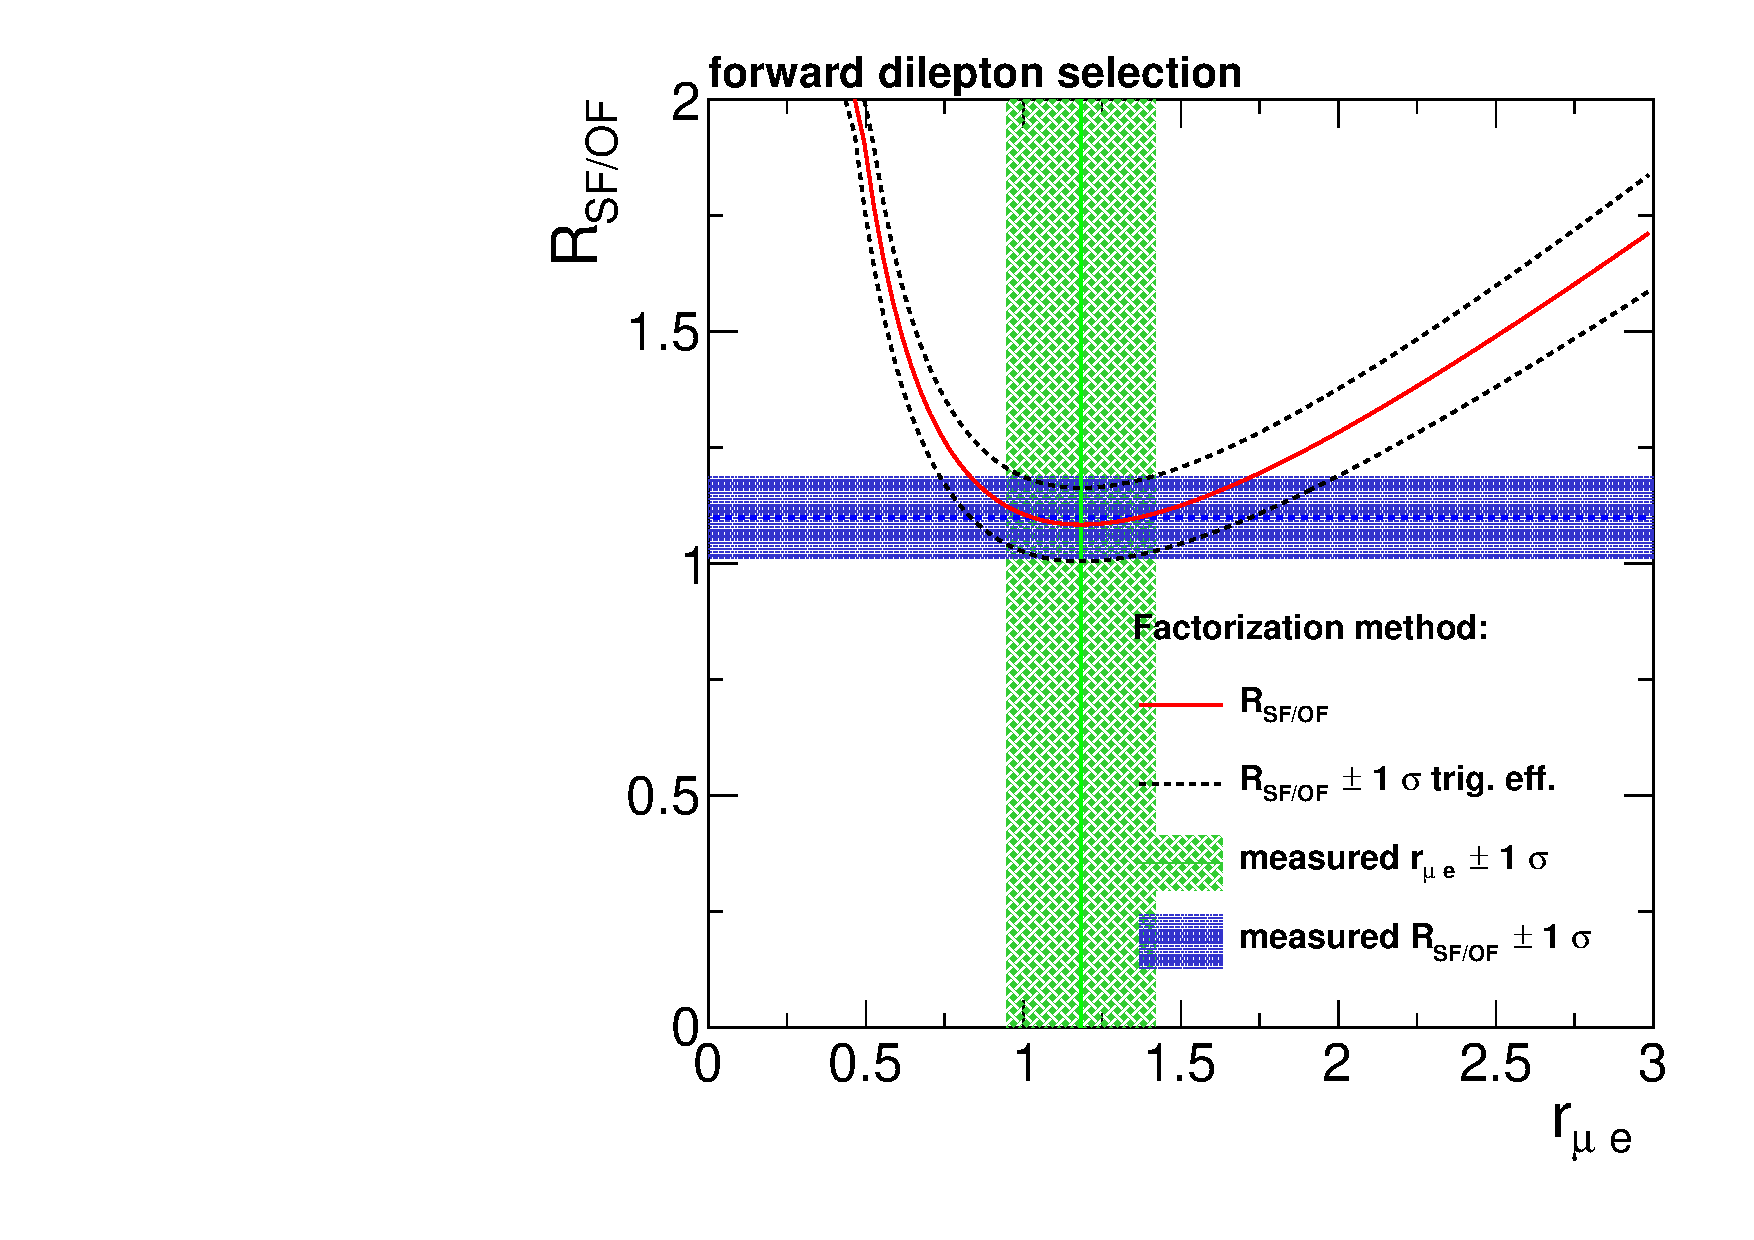
\includegraphics[width=\textwidth]{plots/BG/rmue/rMuEPropaganda_forward.pdf}
\end{minipage}

\caption{Dependency of \Rsfof on \rmue in the factorization method. The measured central values of \Rsfof and \rmue and their uncertainty are shown as the blue and green lines and bands. The red line illustrates the value of \Rsfof for a given \rmue if $R_T$ is kept constant. The impact of a variation of $R_T$ within its uncertainties on \Rsfof is shown by the dashed black lines.}
\label{fig:rmuePropaganda}
\end{figure} 

\subsection{Resulting background estimates}

\begin{table}[hbtp]
 \renewcommand{\arraystretch}{1.3}
 \setlength{\belowcaptionskip}{6pt}
 \scriptsize
 \centering
 \caption{
     }
  \label{tab:combinedRSFOF}
  \begin{tabular}{l| c c| c c }
    & \multicolumn{4}{c}{\Rsfof}  \\ 

    & \multicolumn{2}{c}{Central} & \multicolumn{2}{c}{Forward} \\ 
    								
    \hline
    & Data & MC & Data & MC \
    \hline
        from factorization method       &  1.029\pm0.067  &  1.023\pm0.065      &  1.099\pm0.088 &   1.037\pm0.077    \\
        from direct measurement       &  1.012\pm0.039  &  1.010\pm0.008      &  1.000\pm0.105 &   1.010\pm0.014    \\
        weighted avarage       &  1.016\pm0.034  &  1.010\pm0.008      &  1.034\pm0.052 &   1.011\pm0.014    \\

\hline
    & \multicolumn{4}{c}{\Reeof}  \\ 

    & \multicolumn{2}{c}{Central} & \multicolumn{2}{c}{Forward} \\ 
    								
    \hline
    & Data & MC & Data & MC \
    \hline
        from factorization method       &  0.471\pm0.116  &  0.460\pm0.116      &  0.458\pm0.259 &   0.421\pm0.248    \\
        from direct measurement       &  0.459\pm0.026  &  0.457\pm0.005      &  0.439\pm0.093 &   0.427\pm0.008    \\
        weighted avarage       &  0.459\pm0.023  &  0.457\pm0.005      &  0.439\pm0.038 &   0.427\pm0.008    \\

\hline
    & \multicolumn{4}{c}{\Rmmof}  \\ 

    & \multicolumn{2}{c}{Central} & \multicolumn{2}{c}{Forward} \\ 
    								
    \hline
    & Data & MC & Data & MC \
    \hline
        from factorization method       &  0.558\pm0.117  &  0.563\pm0.118      &  0.641\pm0.261 &   0.617\pm0.250    \\
        from direct measurement       &  0.553\pm0.028  &  0.553\pm0.005      &  0.561\pm0.095 &   0.582\pm0.009    \\
        weighted avarage       &  0.553\pm0.026  &  0.553\pm0.005      &  0.563\pm0.043 &   0.582\pm0.009    \\

\hline
  \end{tabular}
\end{table}


 
\section{Backgrounds containing a Z boson}
To estimate the contribution of backgrounds containing a Z boson to the event sample in the signal region, both the JZB and \MET template methods are used. The first studies the balance of the Z boson against the jets in the event and is therefore called Jet-Z-balance (JZB). In the \MET template method, the \MET distribution of $\gamma$+jets events are used to estimate that of Z+jets events. As the development and application of these methods have not been part of the work covered in this thesis, only a short description will be given. 
\subsection{JZB method}

\section{Investigation of possible further backgrounds}
\section{Search for a kinematic edge with a fit}
